\documentclass[aspectratio=169, 11pt]{beamer}

% ── Theme & Colors ──
\usetheme{Madrid}
\usecolortheme{default}
\definecolor{polimi}{RGB}{26,58,92}
\definecolor{polimired}{RGB}{192,57,43}
\definecolor{polimiblue}{RGB}{41,128,185}
\definecolor{polimigreen}{RGB}{39,174,96}
\definecolor{polimigold}{RGB}{241,196,15}
\setbeamercolor{structure}{fg=polimi}
\setbeamercolor{frametitle}{bg=polimi, fg=white}
\setbeamercolor{title}{fg=white, bg=polimi}
\setbeamercolor{block title}{bg=polimi, fg=white}
\setbeamercolor{block body}{bg=polimi!5}
\setbeamercolor{item}{fg=polimi}
\setbeamertemplate{navigation symbols}{}
\setbeamertemplate{footline}{%
  \leavevmode\hbox{%
    \begin{beamercolorbox}[wd=.33\paperwidth,ht=2.5ex,dp=1ex,left]{author in head/foot}%
      \hspace*{2ex}\insertshortauthor
    \end{beamercolorbox}%
    \begin{beamercolorbox}[wd=.34\paperwidth,ht=2.5ex,dp=1ex,center]{title in head/foot}%
      \insertshorttitle
    \end{beamercolorbox}%
    \begin{beamercolorbox}[wd=.33\paperwidth,ht=2.5ex,dp=1ex,right]{date in head/foot}%
      \insertframenumber{} / \inserttotalframenumber\hspace*{2ex}
    \end{beamercolorbox}%
  }%
}

% ── Packages ──
\usepackage{graphicx}
\usepackage{booktabs}
\usepackage{amsmath}
\usepackage{tikz}
\usepackage{xcolor}
\usepackage{multicol}
\usepackage{adjustbox}

% ── Logo in corner (every slide except title) ──
\addtobeamertemplate{frametitle}{}{%
  \begin{tikzpicture}[remember picture, overlay]
    \node[anchor=north east, yshift=-0.1cm, xshift=-0.2cm]
      at (current page.north east)
      {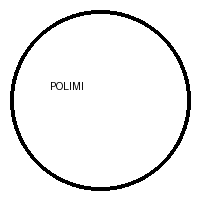
\includegraphics[height=0.9cm]{logo_circle.png}};
  \end{tikzpicture}
}

% ── Metadata ──
\title[EWS for Risk-Off Regimes]{Early-Warning System for Risk-Off Regimes\\with Domain-Specific Allocation Routing}
\subtitle{Unsupervised Anomaly Detection for Regime-Aware Portfolio Allocation}
\author[Ercelli, Galli, Impenati, Mazzini]{Edoardo Ercelli \and Luca Galli \and Francesco Impenati \and Francesco Mazzini}
\institute{POLIMI Graduate School of Management\\Politecnico di Milano}
\date{May 2025}

\begin{document}

% ════════════════════════════════════════════════
% PART I — PRESENTATION
% ════════════════════════════════════════════════

% ── SLIDE 1: COVER ──
{
\setbeamertemplate{footline}{}
\begin{frame}[plain]
\vspace{0.5cm}
\begin{center}
  
\includegraphics[height=2.5cm]{logo_full.png}\\[0.8cm]
  {\Large\bfseries\color{polimi} Early-Warning System for Risk-Off Regimes}\\[0.3cm]
  {\large\color{polimi!80} with Domain-Specific Allocation Routing}\\[0.5cm]
  {\normalsize Unsupervised Anomaly Detection for Regime-Aware Portfolio Allocation}\\[0.8cm]
  \textbf{Edoardo Ercelli\quad$\cdot$\quad Luca Galli\quad$\cdot$\quad Francesco Impenati\quad$\cdot$\quad Francesco Mazzini}\\[0.3cm]
  {\small POLIMI Graduate School of Management --- Politecnico di Milano}\\[0.2cm]
  {\small New Technologies for Finance --- May 2025}
\end{center}
\end{frame}
}

% ── SLIDE 2: PROBLEM STATEMENT ──
\begin{frame}{Problem Statement \& Motivation}
\begin{columns}[T]
\begin{column}{0.55\textwidth}
  \textbf{The gap in traditional risk management:}
  \begin{itemize}
    \item Most early-warning systems treat risk-off as a \textbf{binary decision}: equity vs.\ cash.
    \item But crises are \textit{heterogeneous}: in 2008 the USD was the safe haven (dollar funding squeeze); in 2020 it initially strengthened then weakened; in an inflationary stress regime, \textbf{gold} outperforms.
    \item No existing framework combines \textbf{regime detection} with \textbf{allocation routing} based on the \textit{nature} of the stress.
  \end{itemize}

  \vspace{0.3cm}
  \textbf{Our contribution:}\\
  An EWS that answers \textit{two} questions simultaneously:
  \begin{enumerate}
    \item \textbf{When} to go risk-off (ensemble anomaly detection)
    \item \textbf{Where} to allocate (domain-specific macro routing)
  \end{enumerate}
\end{column}
\begin{column}{0.42\textwidth}
  \textbf{Investment thesis:}\\[0.2cm]
  Deploy \textbf{1.5$\times$ equity leverage} during calm regimes to exploit the equity risk premium, and rely on the EWS to detect stress early enough to \textbf{avoid drawdowns} --- the key to maximizing the Sharpe ratio.\\[0.3cm]
  The leverage is justified only if the detection system has sufficient \textbf{recall}: missing a crisis at 1.5$\times$ is costlier than at 1.0$\times$.\\[0.3cm]

  \footnotesize
  \textit{Key references:}\\
  Maggiori (2020) --- dollar as global safe asset\\
  Baur \& Lucey (2010) --- gold hedge vs.\ safe haven\\
  Avdjiev et al.\ (2019) --- dollar-leverage-flows
\end{column}
\end{columns}
\end{frame}

% ── SLIDE 3: DATASET ──
\begin{frame}{Dataset Overview}
\begin{columns}[T]
\begin{column}{0.48\textwidth}
  \textbf{Source:} Bloomberg weekly data\\
  \textbf{Period:} 2000-01-11 to 2021-04-20 (1{,}111 obs)\\
  \textbf{Target:} $Y=1$ $\Rightarrow$ risk-off week (21.3\% prevalence)\\
  \textbf{Missing values:} None\\[0.3cm]

  \footnotesize
  \begin{tabular}{lrl}
    \toprule
    \textbf{Asset Class} & \textbf{\#} & \textbf{Examples}\\
    \midrule
    Equity (MSCI) & 7 & MXUS, MXEU, MXJP, MXBR\ldots\\
    FX & 3 & DXY, GBP, JPY\\
    Commodities & 4 & Gold, WTI, CRB, Baltic Dry\\
    Bond TR indices & 8 & US/EU/UK/EM Agg, HY, IG\ldots\\
    Yields/rates & 18 & US, DE, GB, IT, JP tenors\\
    Other & 2 & VIX, US Econ Surprise\\
    \bottomrule
  \end{tabular}\\[0.3cm]

  \normalsize
  \textbf{Proxy decisions:}\\
  \footnotesize
  MSCI World (absent) $\rightarrow$ \textbf{MXUS}\\
  Global Aggregate (absent) $\rightarrow$ \textbf{LUACTRUU}\\
  Credit spreads $=$ log price-index ratios (not OAS)
\end{column}
\begin{column}{0.50\textwidth}
  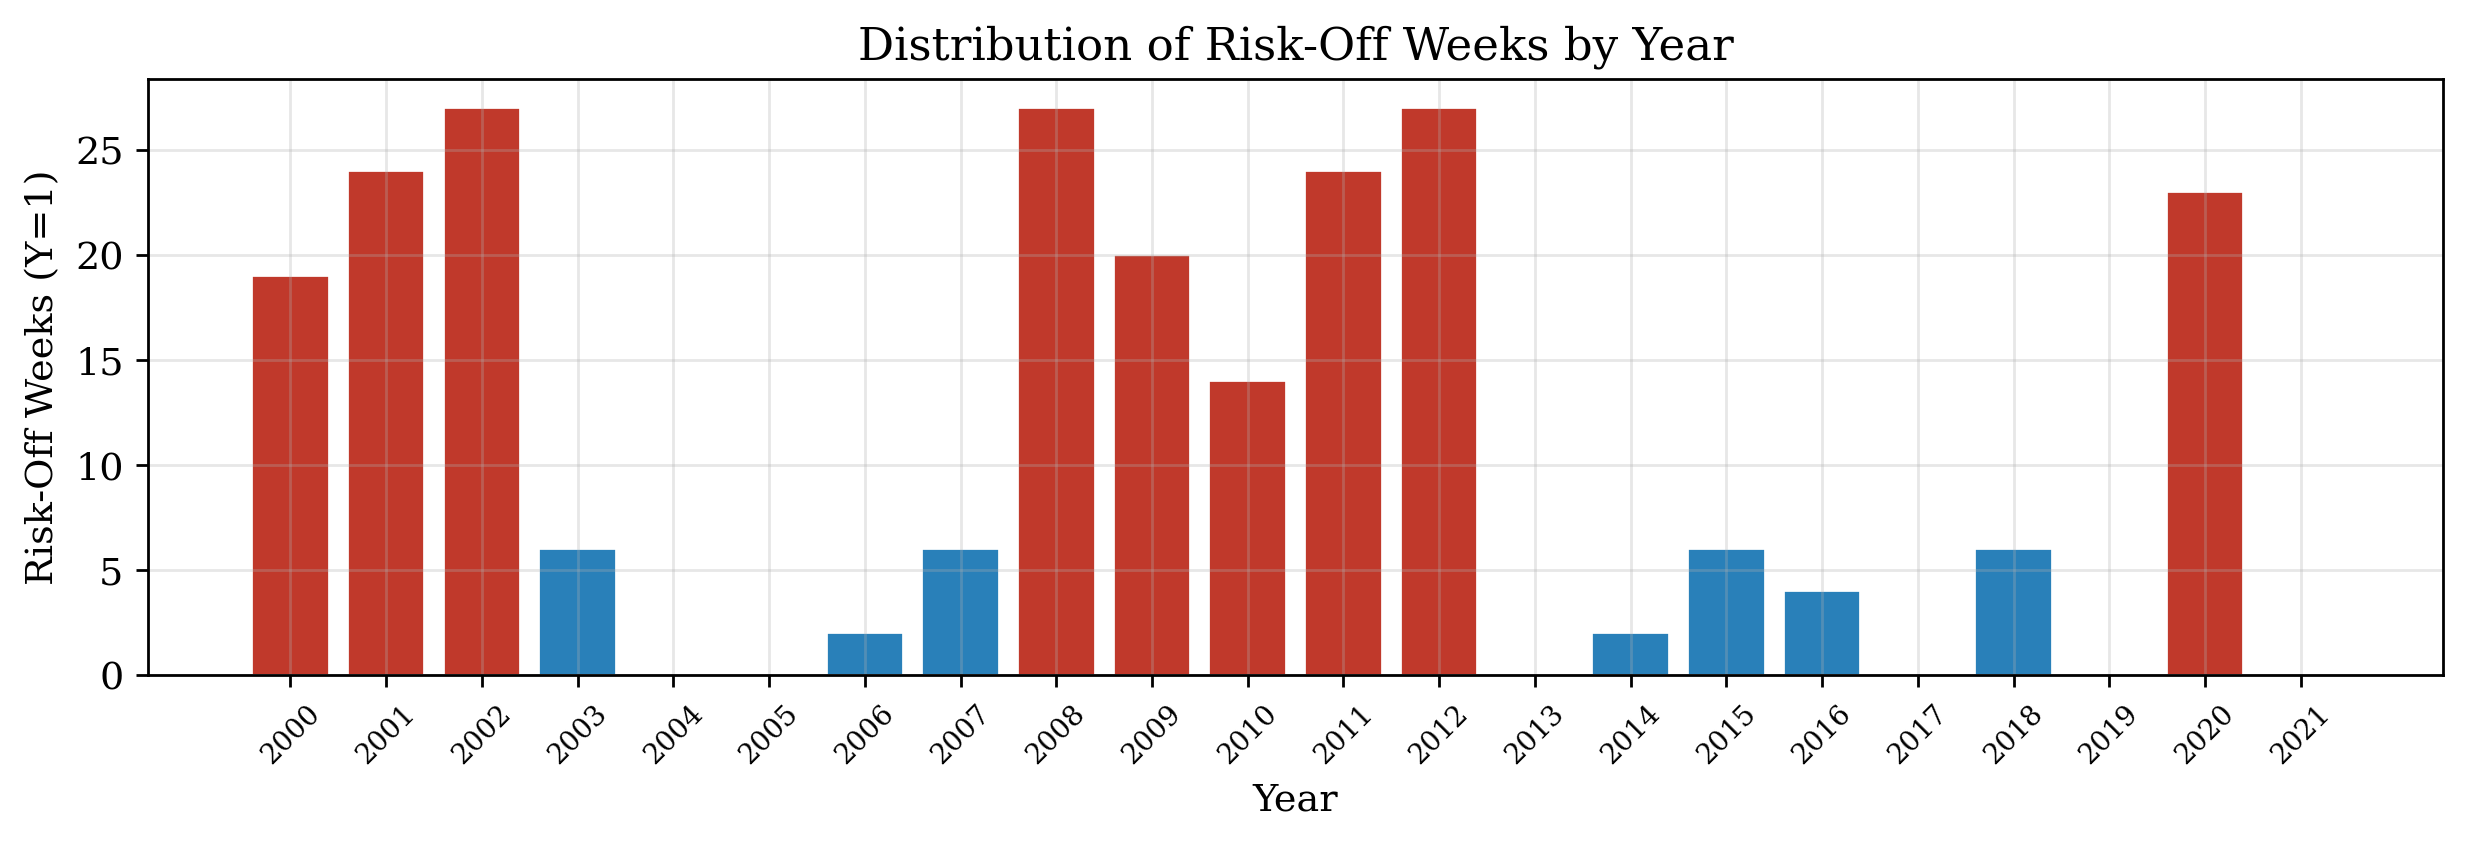
\includegraphics[width=\textwidth]{figures/fig_y_distribution.png}\\[0.2cm]
  \footnotesize
  Risk-off clusters in \textbf{2000--02, 2008--09, 2011--12, 2020}. Mid-decade years (2004--05, 2013, 2017) have zero or near-zero positives --- this is a data property that critically shapes CV design.
\end{column}
\end{columns}
\end{frame}

% ════════════════════════════════════════════════
% PART II — BUSINESS LOGIC
% ════════════════════════════════════════════════

% ── SLIDE 4: THREE MACRO DOMAINS ──
\begin{frame}{Business Logic: Three Macroeconomic Domains for Routing}
\small
\begin{columns}[T]
\begin{column}{0.32\textwidth}
  \textbf{\color{polimiblue}USD Domain}\\[0.15cm]
  \footnotesize
  The dollar is safe haven when stress is \textit{global but external to the US} or when there is a \textbf{dollar funding squeeze} (Avdjiev et al.\ 2019).\\[0.2cm]
  \textbf{Triggers (signed z-scores):}
  \begin{itemize}\setlength\itemsep{0.05cm}
    \item[\color{polimiblue}$+$] LIBOR-3M spread $\Delta_{4w}$
    \item[\color{polimiblue}$+$] DXY momentum $\Delta_{4w}$
    \item[\color{polimiblue}$+$] VRP (implied $>$ realized)
    \item[\color{polimiblue}$-$] US 10Y $\Delta$ change (flight)
    \item[\color{polimiblue}$+$] USA relative vs DM composite
  \end{itemize}
\end{column}
\begin{column}{0.32\textwidth}
  \textbf{\color{polimigold}Gold Domain}\\[0.15cm]
  \footnotesize
  Gold when stress has a \textbf{monetary/inflationary} component or the dollar itself is the problem (Erb \& Harvey 2013; Baur \& Lucey 2010).\\[0.2cm]
  \textbf{Triggers (signed z-scores):}
  \begin{itemize}\setlength\itemsep{0.05cm}
    \item[\color{polimigold}$-$] Real yield proxy $\Delta_{4w}$
    \item[\color{polimigold}$-$] DXY $\Delta_{4w}$ (\textit{opposite sign})
    \item[\color{polimigold}$+$] JPY strength (safe haven)
    \item[\color{polimigold}$+$] Equity-bond $\rho_{13w}$ (diversif.\ failure)
    \item[\color{polimigold}$+$] Gold-oil ratio $\Delta_{4w}$
  \end{itemize}
\end{column}
\begin{column}{0.32\textwidth}
  \textbf{\color{gray}MBS Domain}\\[0.15cm]
  \footnotesize
  MBS is \textit{not} a crisis refuge --- it is \textbf{defensive carry} for moderate stress (Diep et al.\ 2021). Strict activation, conservative by design.\\[0.2cm]
  \textbf{Rule-based activation:}
  \begin{itemize}\setlength\itemsep{0.05cm}
    \item VIX $\in [20, 28]$ (nervous, not panic)
    \item Term spread $> 0$ (normal curve)
    \item Drawdown $\in [-12\%, -5\%]$
  \end{itemize}
  \textbf{Block if:}
  \begin{itemize}\setlength\itemsep{0.05cm}
    \item VIX $> 30$ (acute stress)
    \item Funding spread $>$ p90
    \item HY-IG widening $> 50$bps
  \end{itemize}
\end{column}
\end{columns}
\vspace{0.2cm}
\centering
\footnotesize\textit{Note:} DXY appears in both USD ($+$) and Gold ($-$) domains with opposite sign --- same indicator, opposite economic reading. This is by design.
\end{frame}

% ── SLIDE 5: DECISION MATRIX ──
\begin{frame}{Routing Architecture \& Decision Matrix}
\begin{columns}[T]
\begin{column}{0.52\textwidth}
  \textbf{Allocation Decision Matrix}\\[0.2cm]
  \footnotesize
  \begin{tabular}{llll}
    \toprule
    \textbf{Signal} & \textbf{Condition} & \textbf{Allocation} & \textbf{Weight}\\
    \midrule
    Risk-on (0) & --- & Equity & 1.5$\times$ eq, $-$0.5$\times$ cash\\
    Risk-off (1) & USD $> \tau_u$ \& DXY$\uparrow$ & Cash USD & 1.0$\times$ cash\\
    Risk-off (1) & Gold $> \tau_g$ & Gold & 1.0$\times$ gold\\
    Risk-off (1) & MBS active & MBS & 1.0$\times$ MBS\\
    Risk-off (1) & Default & Cash USD & 1.0$\times$ cash\\
    \bottomrule
  \end{tabular}\\[0.4cm]

  \normalsize
  \textbf{Design principles:}
  \begin{itemize}\setlength\itemsep{0.1cm}
    \item \textbf{Priority ordering:} USD $\rightarrow$ Gold $\rightarrow$ MBS (funding stress is more urgent)
    \item \textbf{Default = Cash:} zero-cost option that doesn't compound errors
    \item \textbf{Transaction costs:} differentiated --- equity 5bps, cash 2bps, gold 8bps, MBS 20bps
  \end{itemize}
\end{column}
\begin{column}{0.46\textwidth}
  \textbf{Sub-score construction:}\\[0.1cm]
  \footnotesize
  For USD and Gold domains:
  \[
    S_d = \frac{1}{|D|} \sum_{f \in D} \text{sign}_f \cdot \frac{x_f - \mu_f^{\text{dev}}}{\sigma_f^{\text{dev}}}
  \]
  where $\mu, \sigma$ are estimated \textbf{only on the development set} (no leakage).\\[0.3cm]

  \normalsize
  \textbf{Threshold optimization:}\\
  \footnotesize
  Grid search $\tau_u \in \{0.5, \ldots, 2.0\}$ $\times$ $\tau_g \in \{0.5, \ldots, 1.5\}$, selecting by \textbf{Calmar ratio} weighted by fold duration on walk-forward CV.\\[0.2cm]

  Only \textit{two scalar thresholds} are optimized; the rest of the routing logic is \textbf{rule-based from macroeconomic rationale} --- this drastically reduces overfitting risk vs.\ a fully data-driven approach.
\end{column}
\end{columns}
\end{frame}

% ════════════════════════════════════════════════
% PART III — PROCESS & EXECUTION
% ════════════════════════════════════════════════

% ── SLIDE 6: FEATURE ENGINEERING ──
\begin{frame}{Feature Engineering: Stationarity \& Cross-Asset Spreads}
\begin{columns}[T]
\begin{column}{0.48\textwidth}
  \textbf{Stationarity transforms}\\[0.1cm]
  \footnotesize
  Anomaly detection models assume a \textit{stable} generating distribution. Non-stationary features violate this assumption fundamentally.
  \begin{itemize}\setlength\itemsep{0.05cm}
    \item \textbf{Log-returns} $\log(x_t/x_{t-1})$: prices (equity, FX, commodities, bond TR)
    \item \textbf{First differences} $\Delta x_t$: yields/rates
    \item \textbf{Level}: VIX, ECSURPUS (already stationary)
  \end{itemize}
  \textbf{Result:} 42/42 features pass ADF at 5\%.\\[0.2cm]

  \textbf{Collinearity cleanup:}\\
  7 features removed ($|\rho| > 0.9$), keeping the more interpretable survivor in each pair.\\[0.1cm]
  \textbf{Final: 56 clean features.}
\end{column}
\begin{column}{0.50\textwidth}
  \textbf{20 cross-asset spreads:}
  \footnotesize
  \begin{itemize}\setlength\itemsep{0.03cm}
    \item \textbf{Term:} US 10Y$-$2Y, DE 10Y$-$2Y, BTP$-$Bund, US$-$DE
    \item \textbf{Credit:} HY-IG, EM (log price ratios)
    \item \textbf{VRP:} $\text{VIX} - \hat\sigma_{\text{realized}}^{4w}(\text{MXUS}) \cdot \sqrt{52} \cdot 100$
    \item \textbf{Equity-bond rotation:} $R^{4w}_{\text{MXUS}} - R^{4w}_{\text{LUACTRUU}}$
    \item \textbf{Gold-oil ratio:} flight-to-quality vs.\ growth
    \item \textbf{JPY strength:} $-\Delta_{4w}\log(\text{JPY})$
  \end{itemize}
  Each spread: level + 4-week change.\\[0.15cm]
  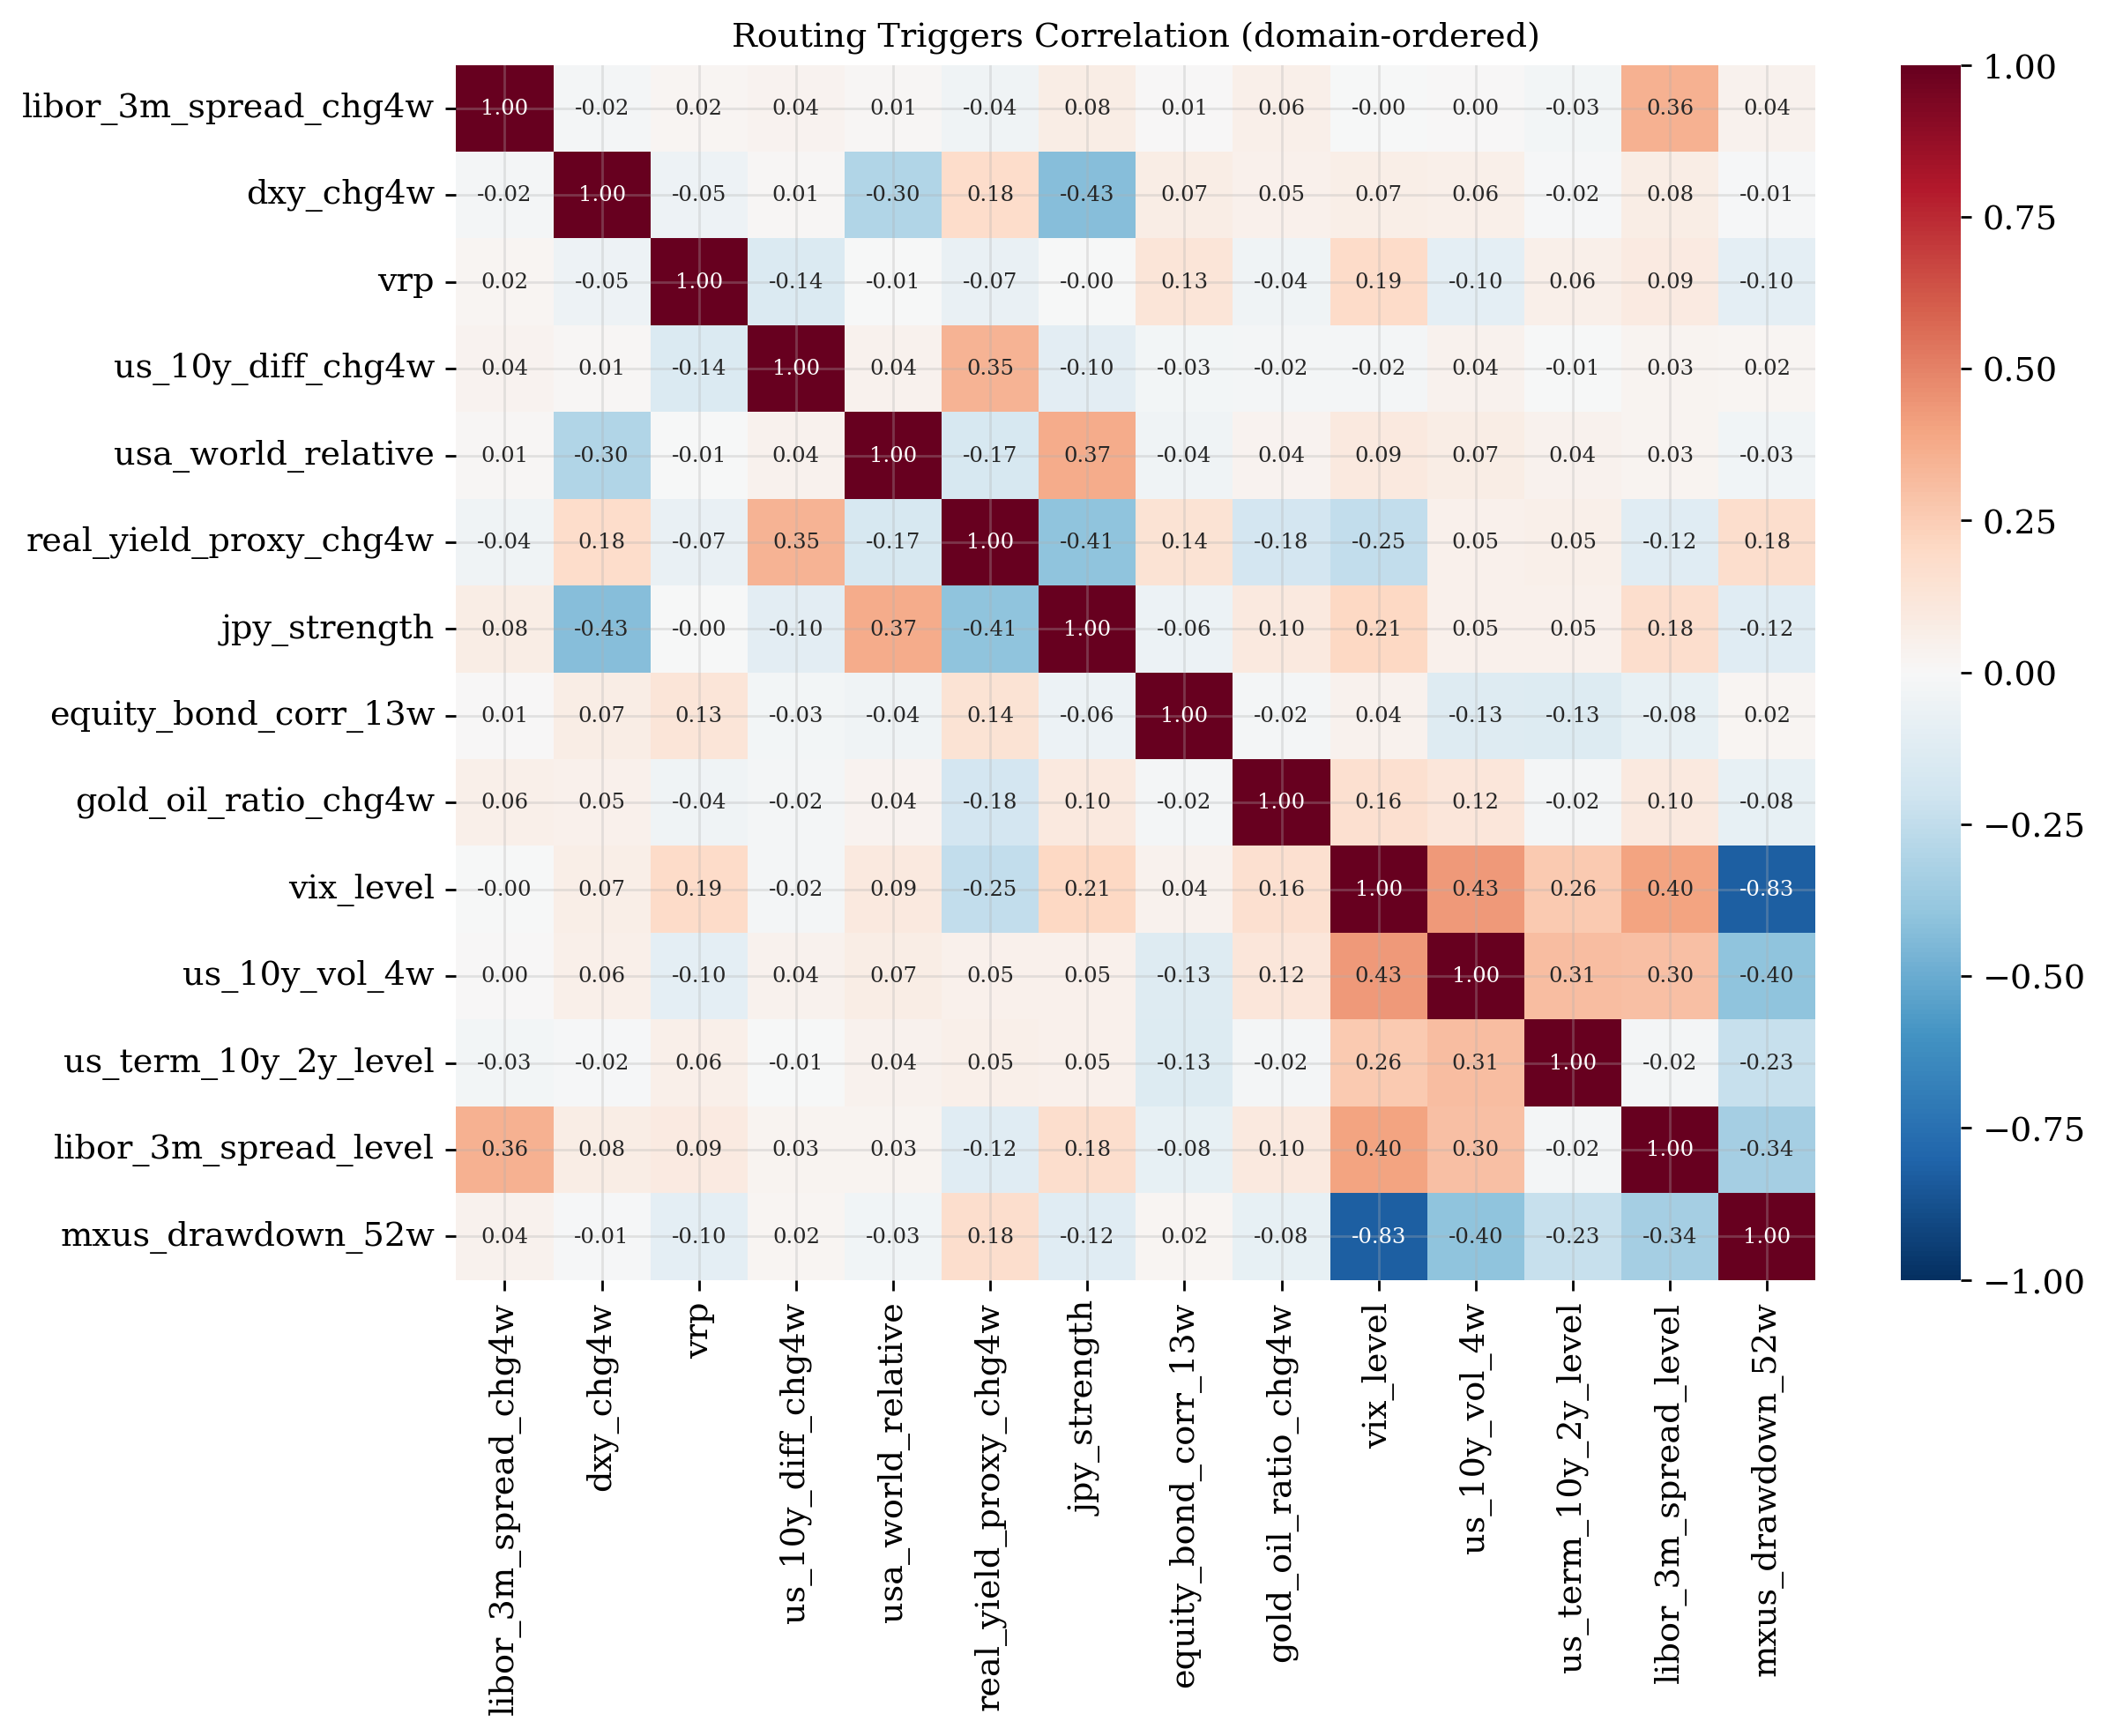
\includegraphics[width=\textwidth]{figures/fig_routing_corr.png}
\end{column}
\end{columns}
\end{frame}

% ── SLIDE 7: WALK-FORWARD CV ──
\begin{frame}{Walk-Forward Cross-Validation with Purged Embargo}
\begin{columns}[T]
\begin{column}{0.55\textwidth}
  \textbf{Design rationale:}
  \begin{itemize}\setlength\itemsep{0.1cm}
    \item \textbf{Expanding window:} train always starts at $t_0$, grows forward --- mimics real deployment where historical data accumulates
    \item \textbf{4-week embargo:} we drop 4 observations between train end and val start. This eliminates leakage from the 4-week lookback features ($\Delta_{4w}$, rolling windows). \textbf{No overlap possible.}
    \item \textbf{Weighted-by-$n_{\text{pos}}$ aggregation:} folds 1--2 have 53/64 positives (statistically reliable); folds 3--5 have only 2/10/6 because 2013--2018 is a low-volatility regime. This is a \textit{data property}. Weighting ensures thin folds contribute at the margin without dominating.
  \end{itemize}

  \textbf{Test holdout (sealed):}\\
  2019-01 $\rightarrow$ 2021-04 (121 weeks, contains COVID).\\
  \textbf{Never touched during model selection or tuning.}
\end{column}
\begin{column}{0.43\textwidth}
  \footnotesize
  \begin{tabular}{ccrrc}
    \toprule
    \textbf{Fold} & \textbf{Val Period} & \textbf{Y=1} & $n_{\text{pos}}$ & \textbf{Crisis}\\
    \midrule
    1 & 2007--2009 & 34.9\% & \textbf{53} & GFC\\
    2 & 2010--2012 & 41.7\% & \textbf{64} & Euro Debt\\
    3 & 2013--2014 & 2.0\% & 2 & Taper\\
    4 & 2015--2016 & 10.1\% & 10 & China-Oil\\
    5 & 2017--2018 & 6.1\% & 6 & Q4 Selloff\\
    \bottomrule
  \end{tabular}\\[0.3cm]

  \normalsize
  \textbf{Scaler discipline:}\\
  \footnotesize
  \texttt{StandardScaler} fit \textbf{only on each fold's train}. Test holdout scaled with scaler fit on \textit{entire development set}. Autoencoder early stopping uses a \textbf{temporal sub-split of train} --- never the validation fold.\\[0.2cm]
  This is the \#1 source of silent leakage in ML finance papers.
\end{column}
\end{columns}
\end{frame}

% ── SLIDE 8: MODELS ──
\begin{frame}{Four Anomaly Detection Models}
\small
\textbf{Paradigm:} Novelty detection --- models see \textit{only normal weeks} ($Y{=}0$) during training. They learn what ``normal'' looks like; anything sufficiently different is flagged as risk-off.

\vspace{0.2cm}
\begin{columns}[T]
\begin{column}{0.48\textwidth}
\textbf{1. Multivariate Gaussian (MVG)}\\
\footnotesize
Score $= d^2_M(\mathbf{x}) = (\mathbf{x}-\hat{\boldsymbol\mu})^\top \hat{\boldsymbol\Sigma}^{-1} (\mathbf{x}-\hat{\boldsymbol\mu})$\\[0.1cm]
\textbf{Ledoit-Wolf shrinkage} is mandatory: with 56 features and $\sim$360 normals in Fold~1, the sample covariance $\hat\Sigma$ is near-singular. Ledoit-Wolf computes the optimal convex combination $\hat\Sigma^* = (1{-}\alpha)\hat\Sigma + \alpha \cdot \frac{\text{tr}(\hat\Sigma)}{p}\mathbf{I}$ that minimizes expected loss under Frobenius norm, producing a well-conditioned estimator.\\[0.2cm]

\textbf{2. One-Class SVM (RBF)}\\
\footnotesize
Maps normals to a high-dimensional feature space via RBF kernel and finds the smallest hypersphere containing them. Score $= -f(\mathbf{x})$. Grid-searched: $\nu \in \{0.05, 0.10, 0.15, 0.22\}$, $\gamma \in \{\text{scale, auto, 0.01, 0.001}\}$. Best: $\nu{=}0.05, \gamma{=}0.001$.
\end{column}
\begin{column}{0.48\textwidth}
\textbf{3. Autoencoder}\\
\footnotesize
Symmetric bottleneck: $56 \!\to\! 24 \!\to\! 12 \!\to\! 6 \!\to\! 12 \!\to\! 24 \!\to\! 56$.\\
ReLU, dropout 0.15, Adam lr$=$1e-3, MSE loss.\\
Score $= \frac{1}{p}\|\mathbf{x} - \hat{\mathbf{x}}\|^2$.\\
Early stopping on \textbf{temporal 85/15 sub-split of train normals} (never on CV val --- that would leak).\\[0.2cm]
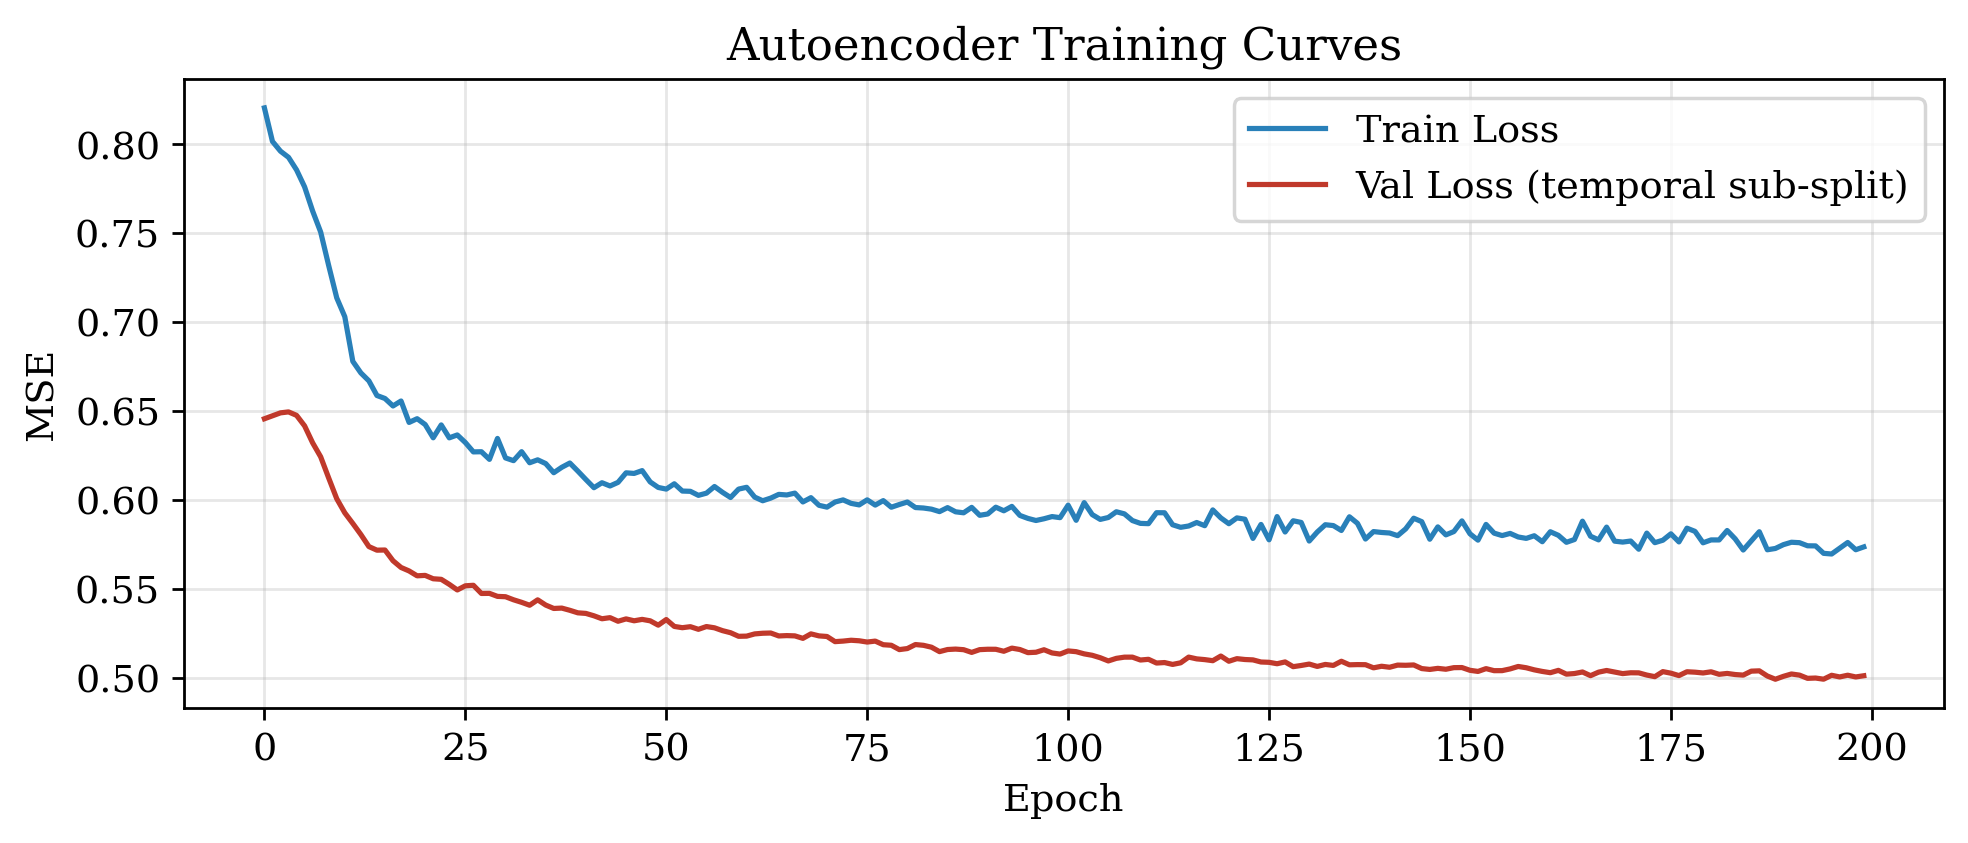
\includegraphics[width=0.95\textwidth]{figures/fig_ae_training.png}\\[0.2cm]

\textbf{4. Isolation Forest}\\
\footnotesize
200 trees, random partitioning. Anomalies are isolated in fewer splits. Grid: contamination $\in \{0.05, 0.10, 0.15, 0.22\}$. Best: 0.10. Threshold fine-tuned via walk-forward.
\end{column}
\end{columns}
\end{frame}

% ── SLIDE 9: MODEL RESULTS ──
\begin{frame}{Model Results (Test Holdout 2019--2021)}
\begin{columns}[T]
\begin{column}{0.48\textwidth}
  \footnotesize
  \begin{tabular}{lcccccc}
    \toprule
    & \textbf{F1} & \textbf{AUC-ROC} & \textbf{AUC-PR} & \textbf{Prec} & \textbf{Rec} & \textbf{F2}\\
    \midrule
    MVG & 0.516 & \textbf{0.886} & \textbf{0.770} & 1.000 & 0.348 & 0.400\\
    SVM & \textbf{0.615} & 0.851 & 0.732 & 0.750 & 0.522 & 0.556\\
    IF & 0.583 & 0.810 & 0.680 & 0.560 & 0.609 & 0.598\\
    AE & 0.516 & 0.873 & 0.764 & 1.000 & 0.348 & 0.400\\
    \bottomrule
  \end{tabular}\\[0.3cm]

  \normalsize
  \textbf{Key observations:}
  \begin{itemize}\setlength\itemsep{0.05cm}
    \footnotesize
    \item MVG and AE: \textbf{perfect precision}, low recall --- when they flag risk-off they're right, but miss most events
    \item SVM: best single model on F1 (balanced)
    \item IF: highest recall (catches 61\% of risk-off weeks)
    \item MVG has highest AUC-ROC (0.886) --- the \textit{ranking} is good; the threshold is conservative
    \item F2 ($\beta{=}2$) weighs recall double: \textbf{missing a crisis at 1.5$\times$ is costlier than a false alarm}
  \end{itemize}
\end{column}
\begin{column}{0.50\textwidth}
  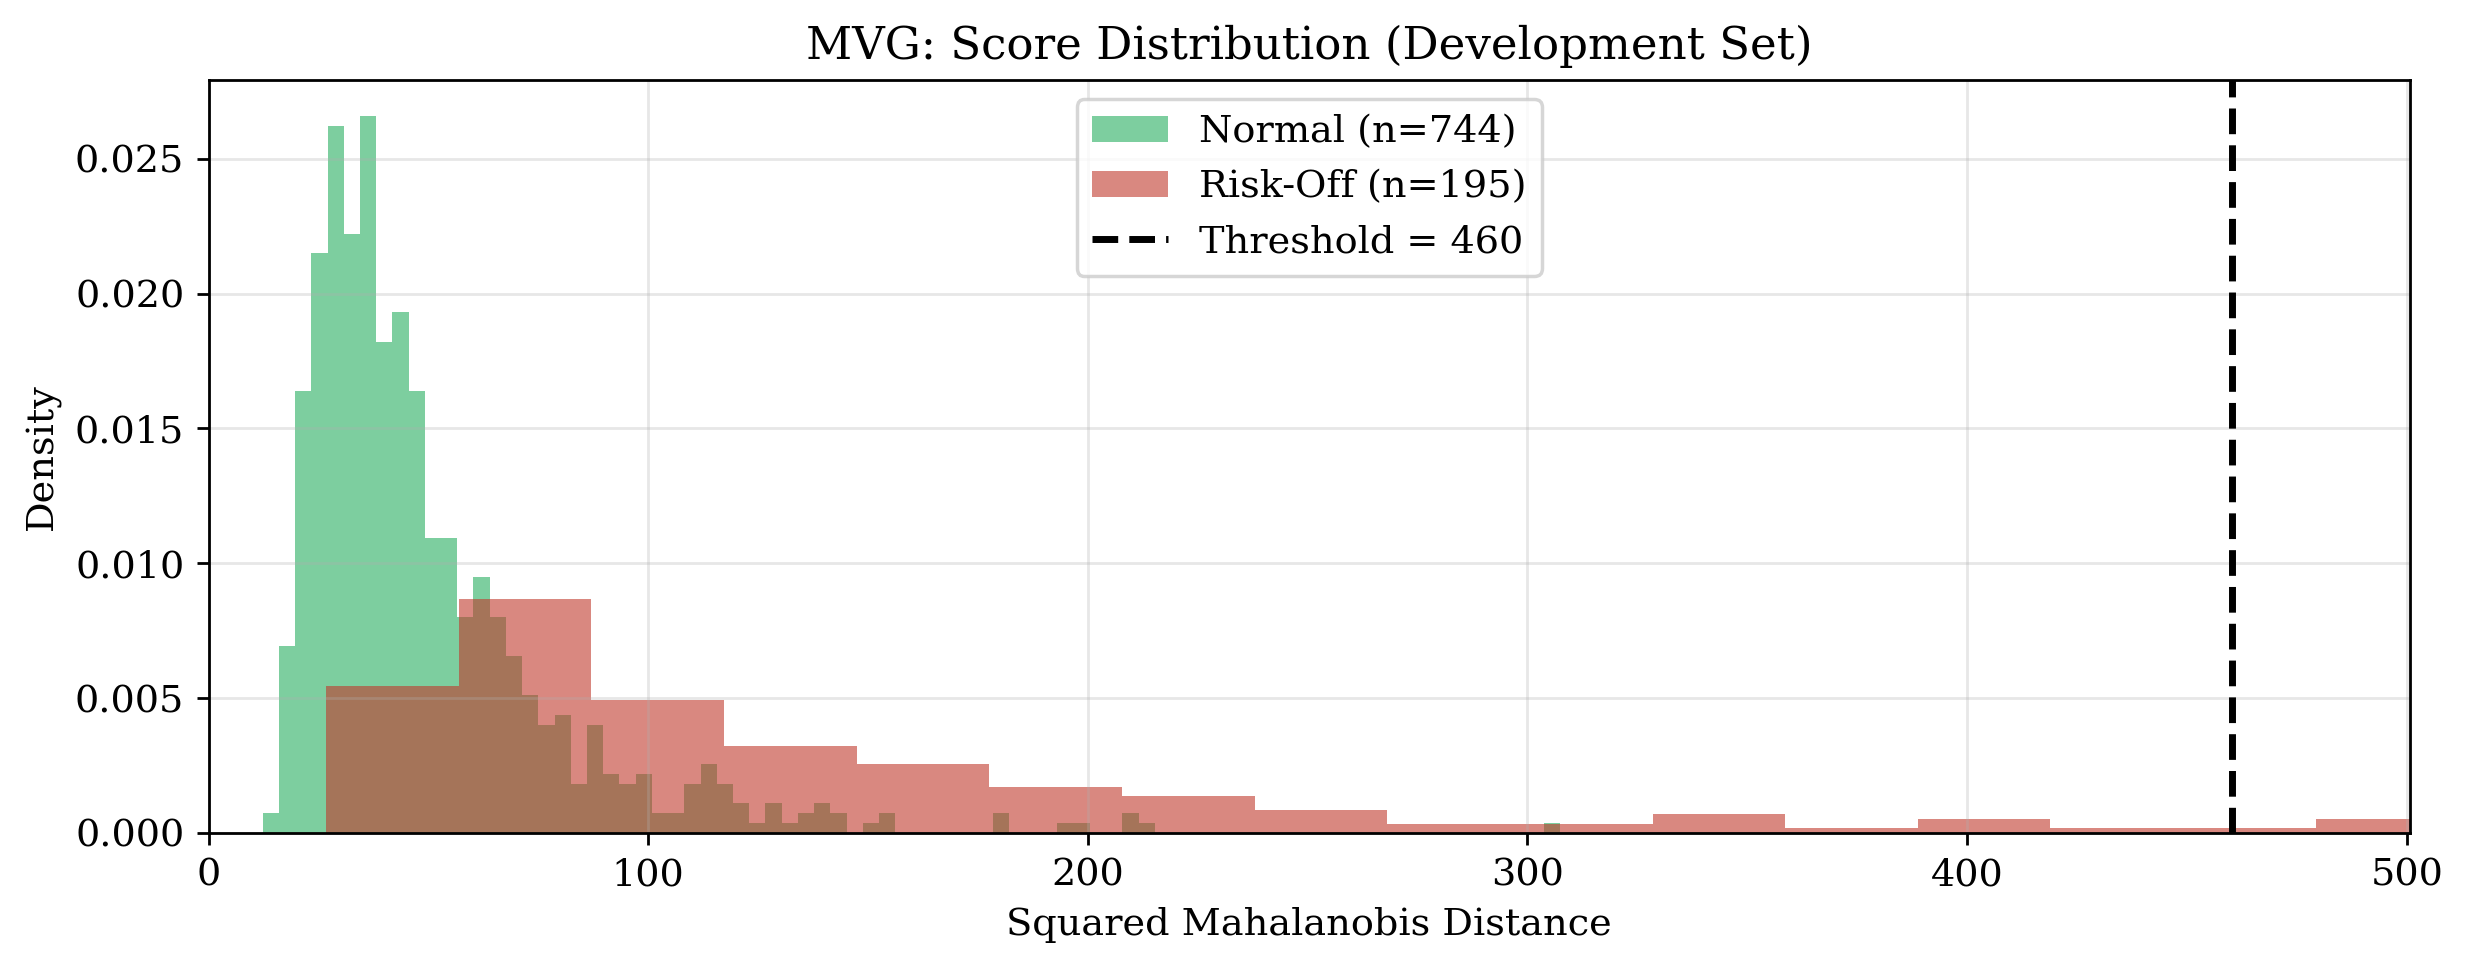
\includegraphics[width=\textwidth]{figures/fig_mvg_scores.png}\\[0.15cm]
  \footnotesize\centering MVG: Mahalanobis distance separates normal (green) from risk-off (red).\\
  Threshold tuned via weighted walk-forward CV.
\end{column}
\end{columns}
\end{frame}

% ── SLIDE 10: ENSEMBLE ──
\begin{frame}{Ensemble: Combining Four Diverse Detectors}
\begin{columns}[T]
\begin{column}{0.55\textwidth}
  \textbf{Why ensemble?}\\
  \footnotesize Each model captures different aspects of anomaly: MVG detects distributional shift, SVM finds boundary violations, AE catches reconstruction difficulty, IF identifies structural isolation. If their errors are \textit{uncorrelated}, combining them reduces both FP and FN.\\[0.2cm]

  \normalsize\textbf{Percentile mapping:}\\
  \footnotesize Raw scores are on incomparable scales. We convert each to its \textbf{empirical percentile} against the train-normals distribution: $p_i = F_{\text{train}}(s_i)$. This makes all scores $\in [0,1]$ with comparable semantics.\\[0.2cm]

  \normalsize\textbf{Three variants:}
  \begin{enumerate}\setlength\itemsep{0.05cm}
    \footnotesize
    \item \textbf{Hard voting:} each model flags 0/1 with own threshold; majority ($\geq$3/4) wins
    \item \textbf{Soft mean:} $\bar{p} = \frac{1}{4}\sum p_i$, threshold $\tau$ tuned on CV
    \item \textbf{Soft median:} $\tilde{p} = \text{median}(p_i)$, robust to one rogue model
  \end{enumerate}
  \textbf{Winner: Soft Mean} (F1=0.650, beats best single 0.615).
\end{column}
\begin{column}{0.43\textwidth}
  \footnotesize
  \begin{tabular}{lccc}
    \toprule
    & \textbf{F1} & \textbf{AUC-ROC} & \textbf{AUC-PR}\\
    \midrule
    MVG & 0.516 & 0.886 & 0.770\\
    SVM & 0.615 & 0.851 & 0.732\\
    IF & 0.583 & 0.810 & 0.680\\
    AE & 0.516 & 0.873 & 0.764\\
    \midrule
    Hard Vote & 0.516 & 0.859 & 0.742\\
    \textbf{Soft Mean} & \textbf{0.650} & 0.859 & 0.742\\
    Soft Median & 0.619 & 0.869 & 0.759\\
    \bottomrule
  \end{tabular}\\[0.3cm]
  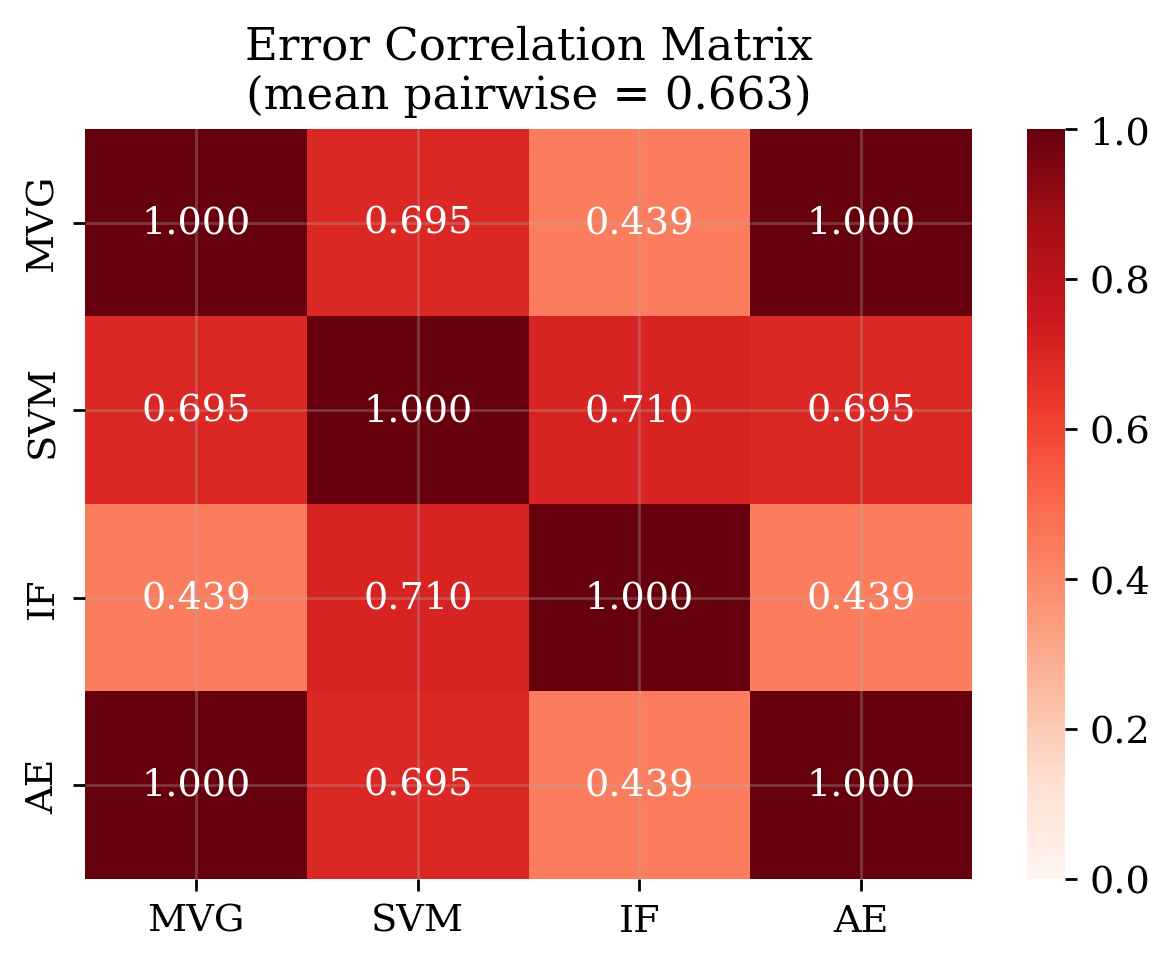
\includegraphics[width=\textwidth]{figures/fig_error_corr.png}\\[0.1cm]
  \footnotesize Mean pairwise error correlation = 0.66 $< 0.85$\\
  $\Rightarrow$ \textbf{Ensemble adds genuine value.}
\end{column}
\end{columns}
\end{frame}

% ── SLIDE 11: ENSEMBLE TIMELINE ──
\begin{frame}{Ensemble Predictions on Test Holdout}
\centering
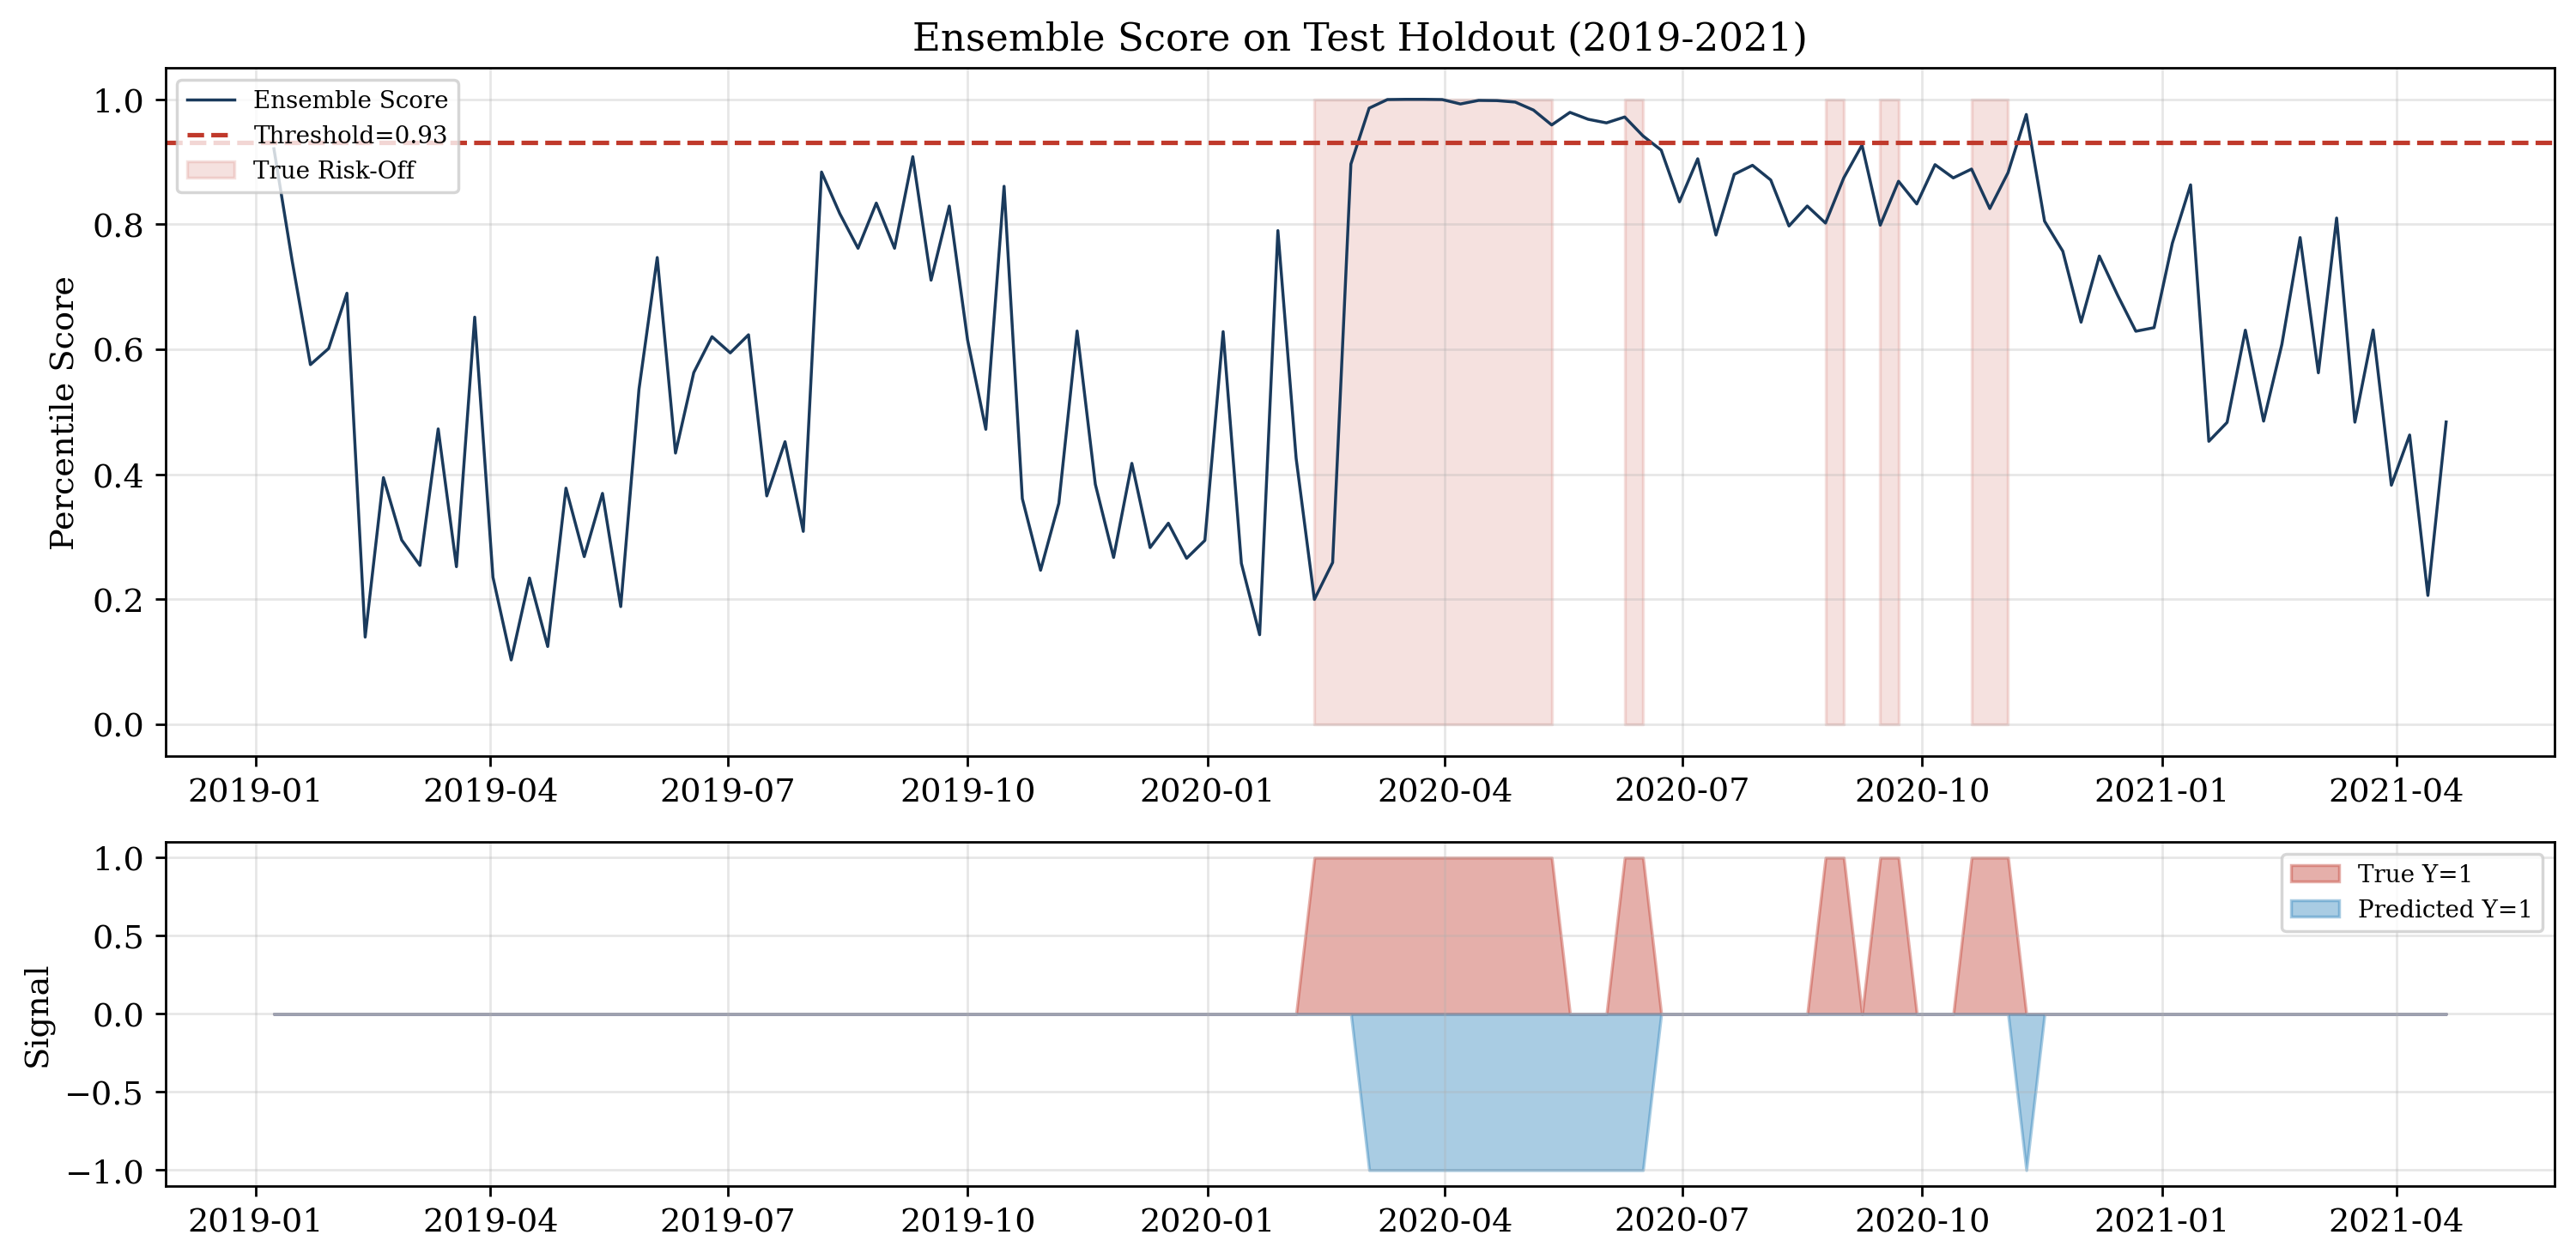
\includegraphics[width=0.92\textwidth]{figures/fig_ensemble_timeline.png}\\[0.2cm]
\footnotesize
\textbf{Top:} Soft mean percentile score vs.\ threshold. Red shading = true risk-off weeks.\\
\textbf{Bottom:} Predicted vs.\ actual signals. The ensemble captures the COVID cluster and filters calm periods.
\end{frame}

% ── SLIDE 12: BACKTEST ──
\begin{frame}{Backtest Results: Strategy vs.\ Benchmarks (2019--2021)}
\begin{columns}[T]
\begin{column}{0.55\textwidth}
  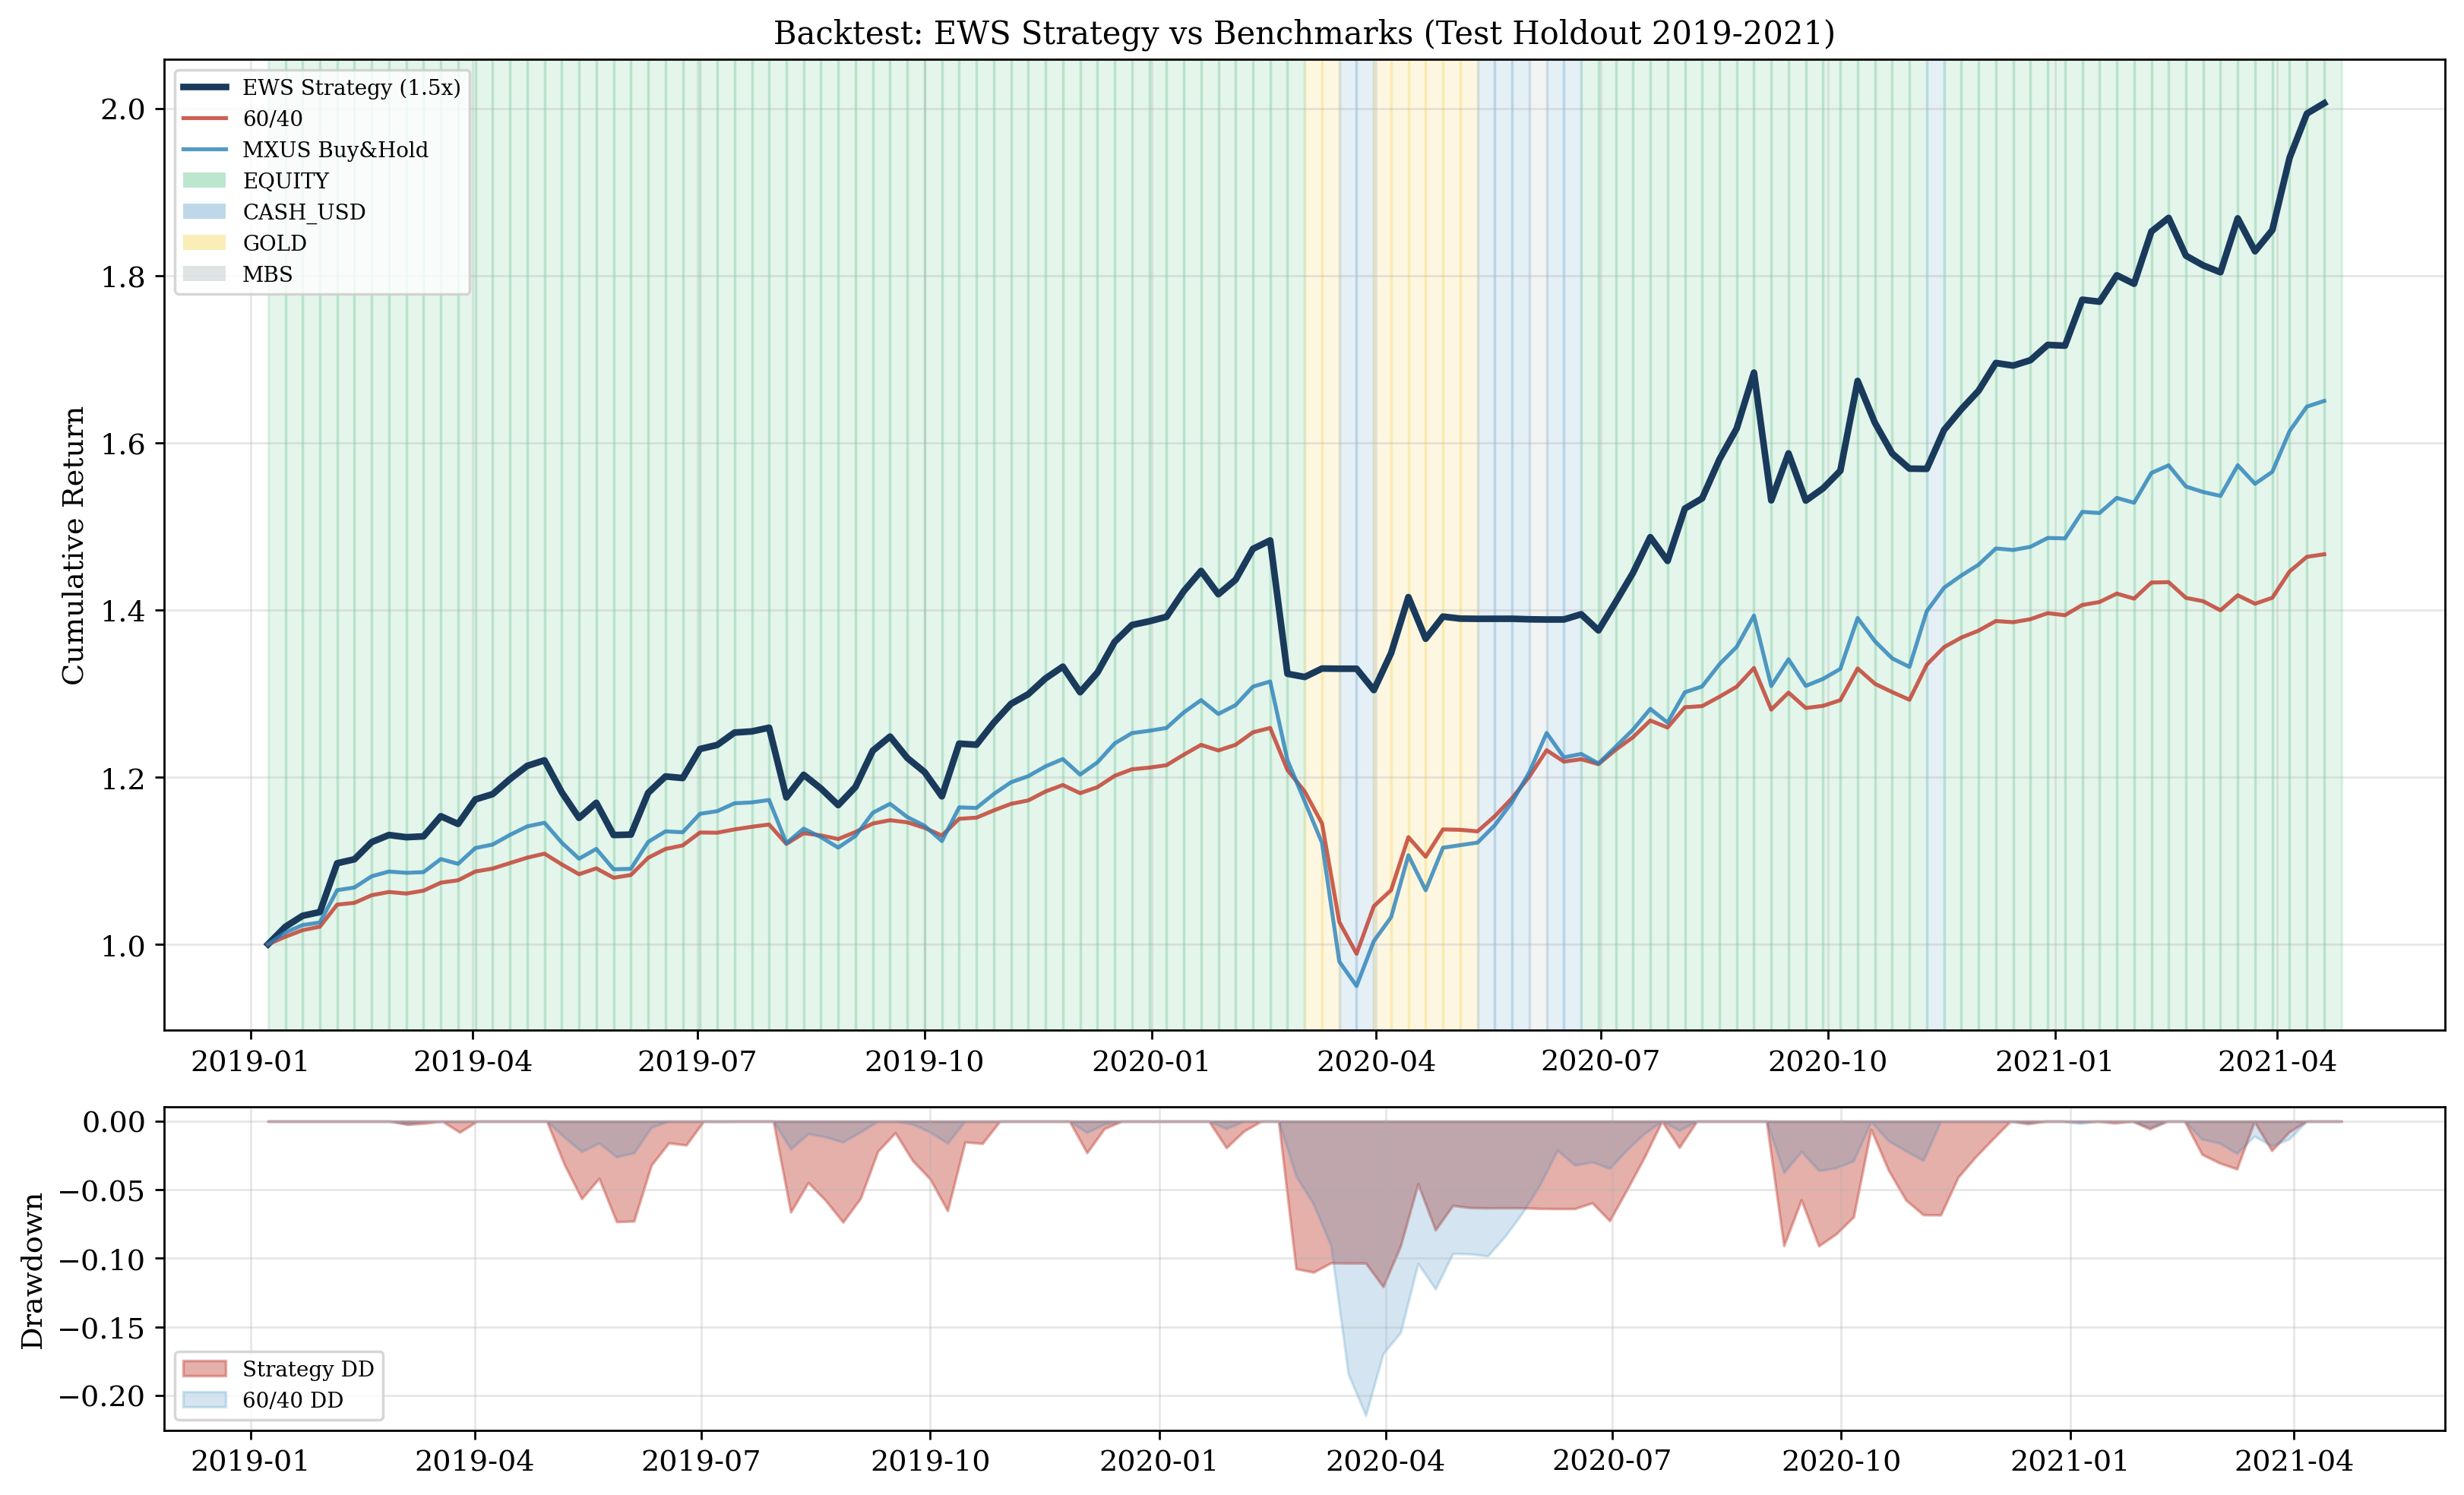
\includegraphics[width=\textwidth]{figures/fig_equity_curves.png}
\end{column}
\begin{column}{0.43\textwidth}
  \footnotesize
  \begin{tabular}{lccc}
    \toprule
    & \textbf{Strategy} & \textbf{60/40} & \textbf{B\&H}\\
    \midrule
    CAGR & \textbf{35.2\%} & 18.1\% & 24.2\%\\
    Sharpe & \textbf{1.93} & 1.44 & 1.38\\
    Max DD & \textbf{$-$12.1\%} & $-$21.5\% & $-$27.7\%\\
    Calmar & \textbf{2.92} & 0.84 & 0.87\\
    Sortino & \textbf{2.10} & --- & ---\\
    Turnover & 3.9/yr & --- & ---\\
    \bottomrule
  \end{tabular}\\[0.3cm]

  \normalsize\textbf{Allocation breakdown:}\\
  \footnotesize
  \begin{tabular}{lr}
    Levered Equity & 103 weeks (85.8\%)\\
    Gold & 8 weeks (6.7\%)\\
    Cash USD & 8 weeks (6.7\%)\\
    MBS & 1 week (0.8\%)\\
  \end{tabular}\\[0.2cm]

  \normalsize\textbf{Key insight:}\\
  \footnotesize
  The leverage generates alpha in calm periods (103 weeks at 1.5$\times$), while the EWS limits drawdowns to $-$12\% vs.\ $-$28\% for buy\&hold. This is exactly the thesis: \textbf{leverage + early warning = superior Sharpe}.
\end{column}
\end{columns}
\end{frame}

% ── SLIDE 13: COVID STRESS TEST ──
\begin{frame}{COVID Stress Test: Trigger Analysis \& Allocation Routing}
\begin{columns}[T]
\begin{column}{0.55\textwidth}
  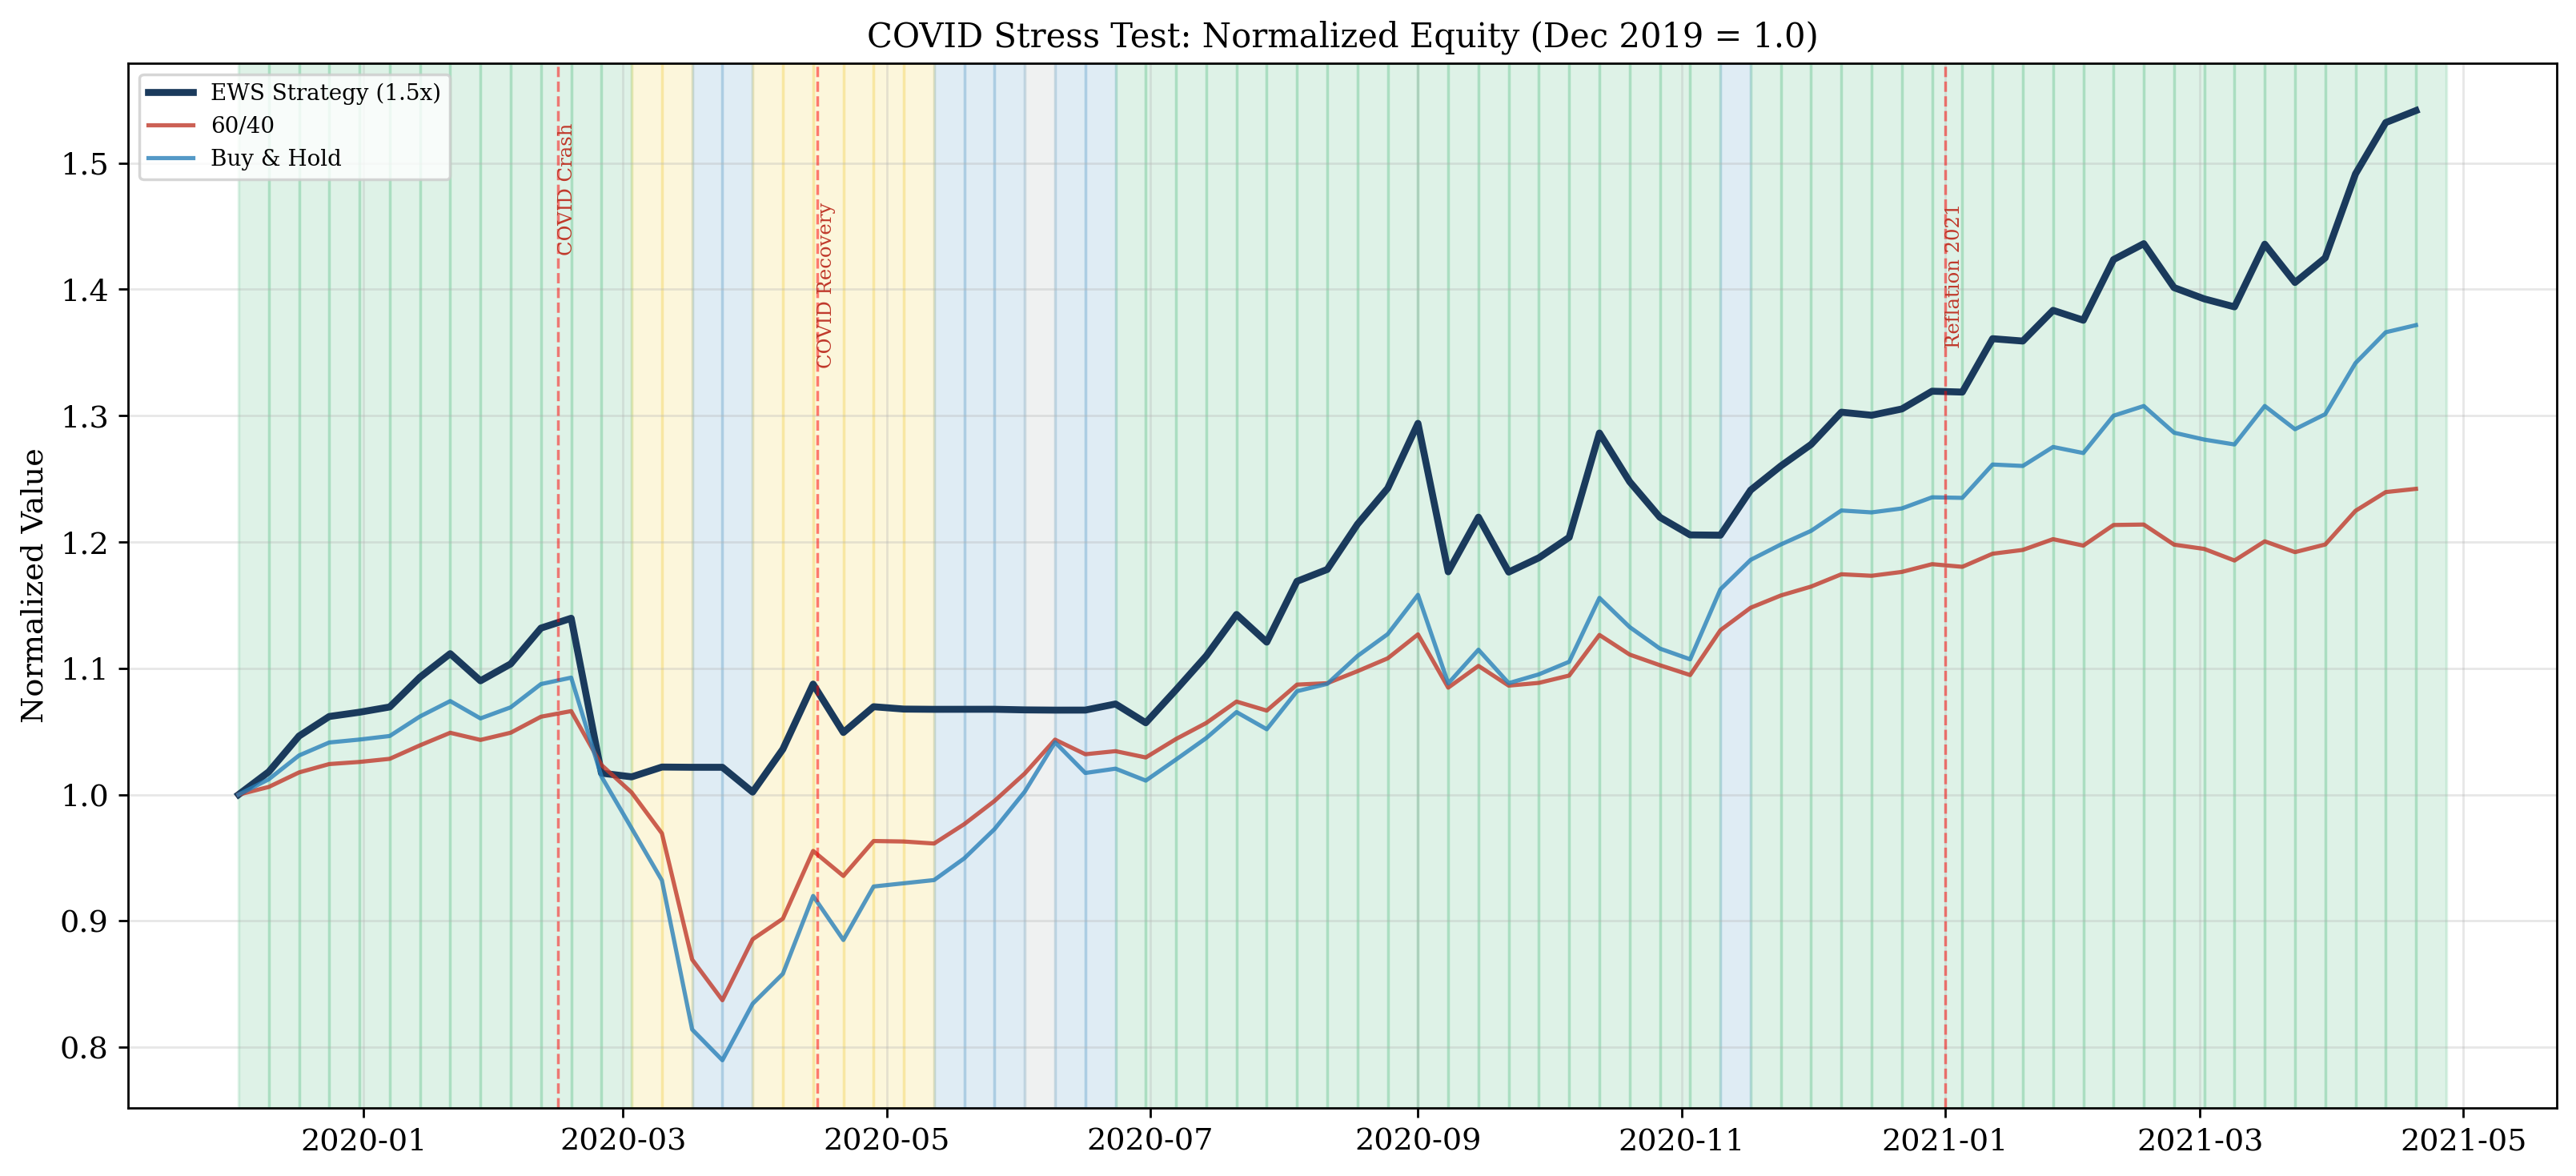
\includegraphics[width=\textwidth]{figures/fig_stress_timeline.png}\\[0.1cm]
  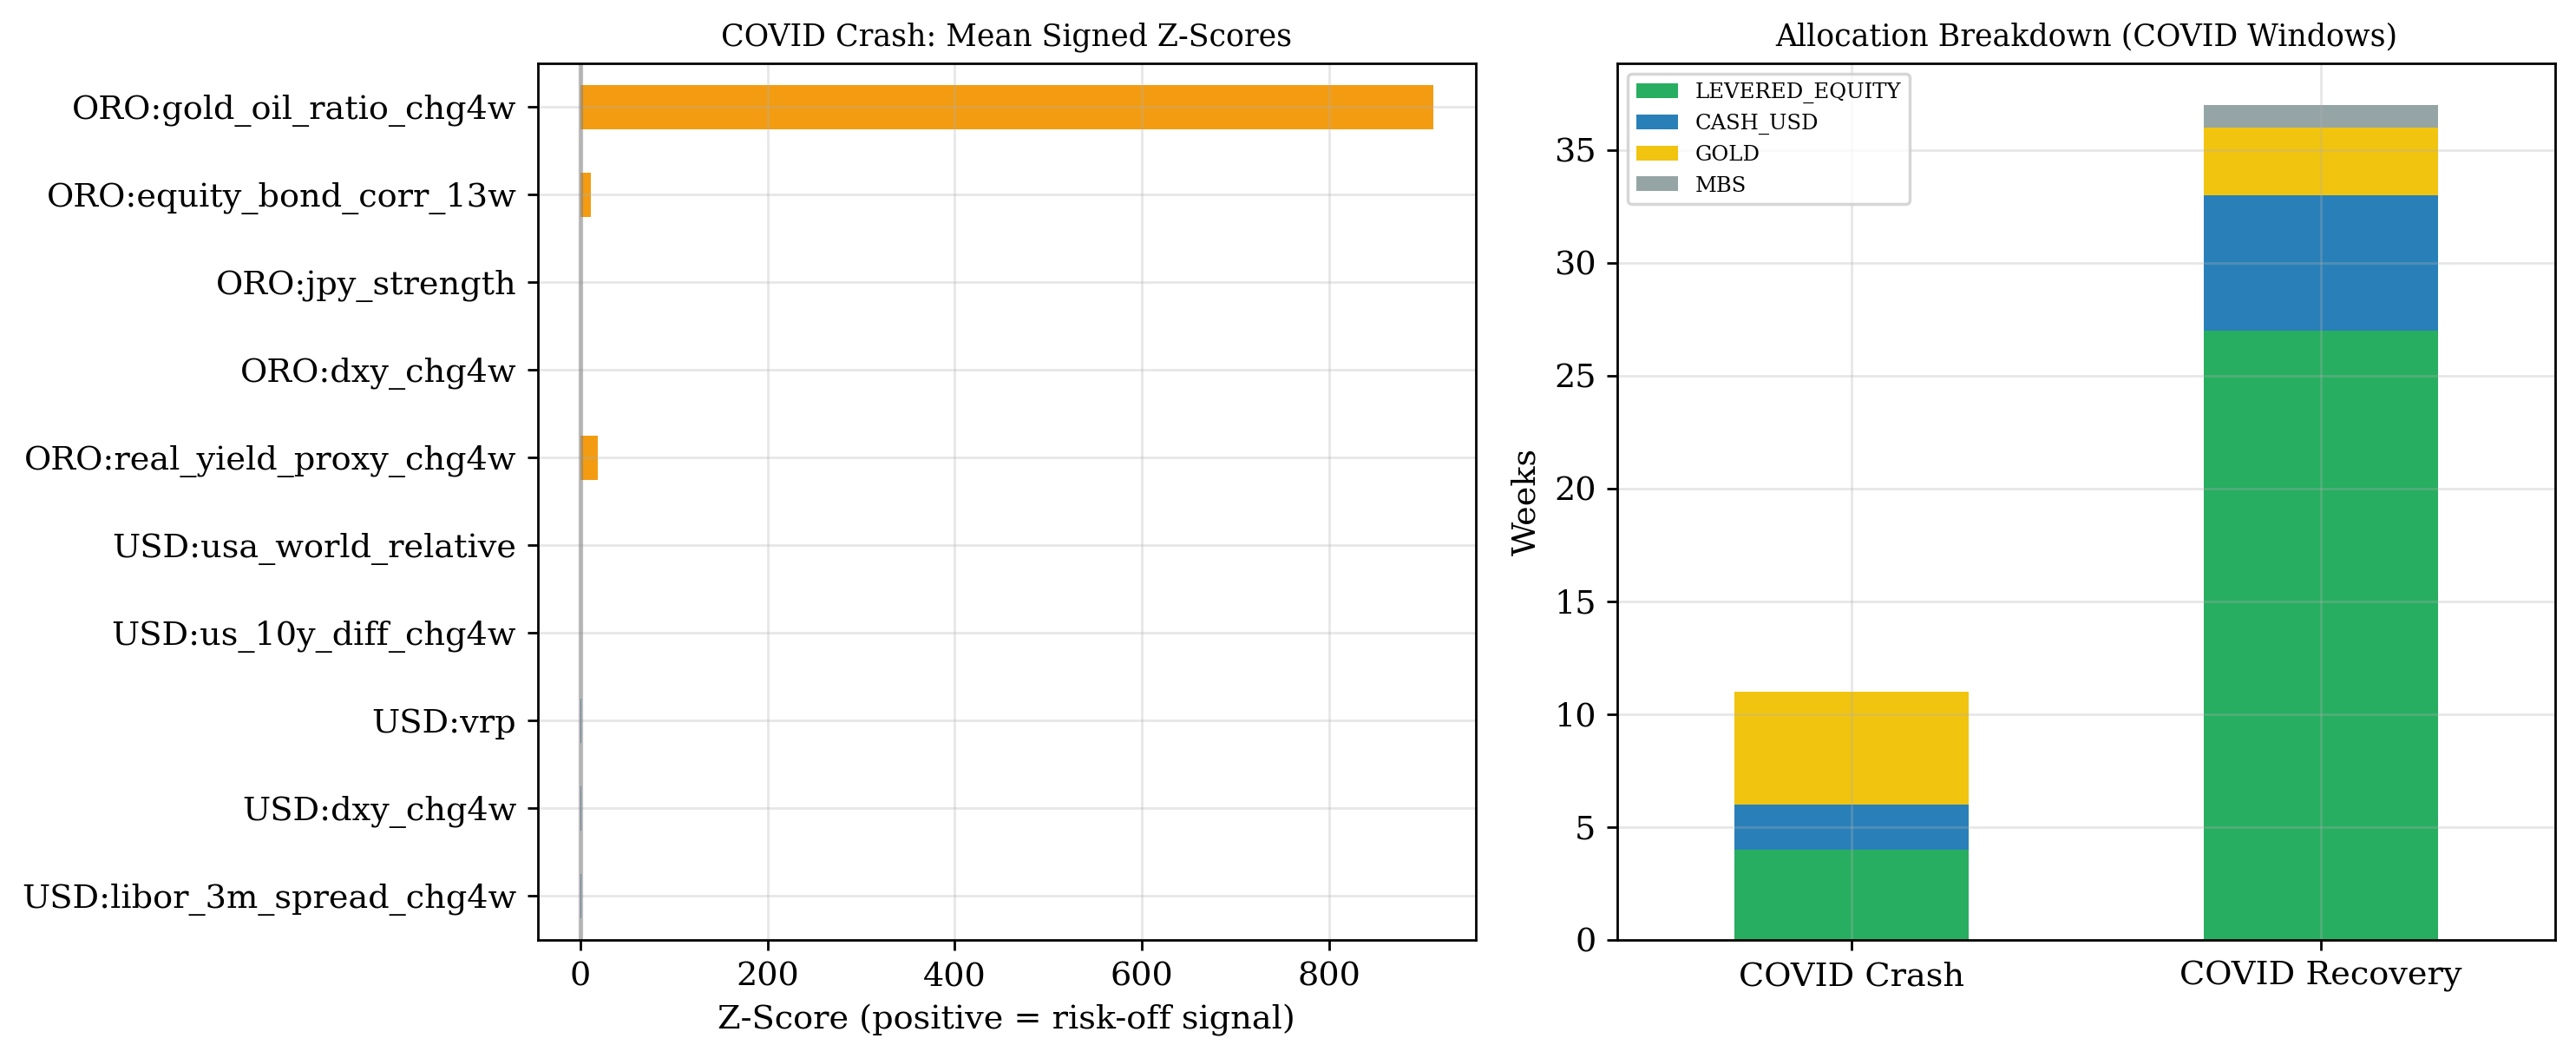
\includegraphics[width=\textwidth]{figures/fig_covid_triggers.png}
\end{column}
\begin{column}{0.43\textwidth}
  \textbf{COVID Crash (Feb--Apr 2020):}\\
  \footnotesize
  \begin{itemize}\setlength\itemsep{0.03cm}
    \item Ensemble signals risk-off as VIX spikes and equity drops
    \item \textbf{USD triggers fire first}: funding stress (LIBOR-3M spread widens), DXY rallies, VRP explodes --- classic dollar squeeze
    \item Routing sends allocation to \textbf{Cash USD and Gold}
    \item MBS correctly \textbf{blocked} (VIX $>$ 30)
  \end{itemize}
  \vspace{0.2cm}

  \normalsize\textbf{COVID Recovery (Apr--Dec 2020):}\\
  \footnotesize
  \begin{itemize}\setlength\itemsep{0.03cm}
    \item Risk-off signals fade as markets stabilize
    \item System returns to \textbf{1.5$\times$ equity}, capturing the V-shaped rebound
    \item Gold score remains elevated (fiscal stimulus $\Rightarrow$ inflation expectations)
  \end{itemize}
  \vspace{0.2cm}

  \normalsize\textbf{Reflation 2021:}\\
  \footnotesize
  \begin{itemize}\setlength\itemsep{0.03cm}
    \item Full equity exposure maintained
    \item No false alarms during re-opening rally
  \end{itemize}
\end{column}
\end{columns}
\end{frame}

% ── SLIDE 14: THRESHOLD OPTIMIZATION ──
\begin{frame}{Threshold Optimization \& Sub-Score Dynamics}
\begin{columns}[T]
\begin{column}{0.48\textwidth}
  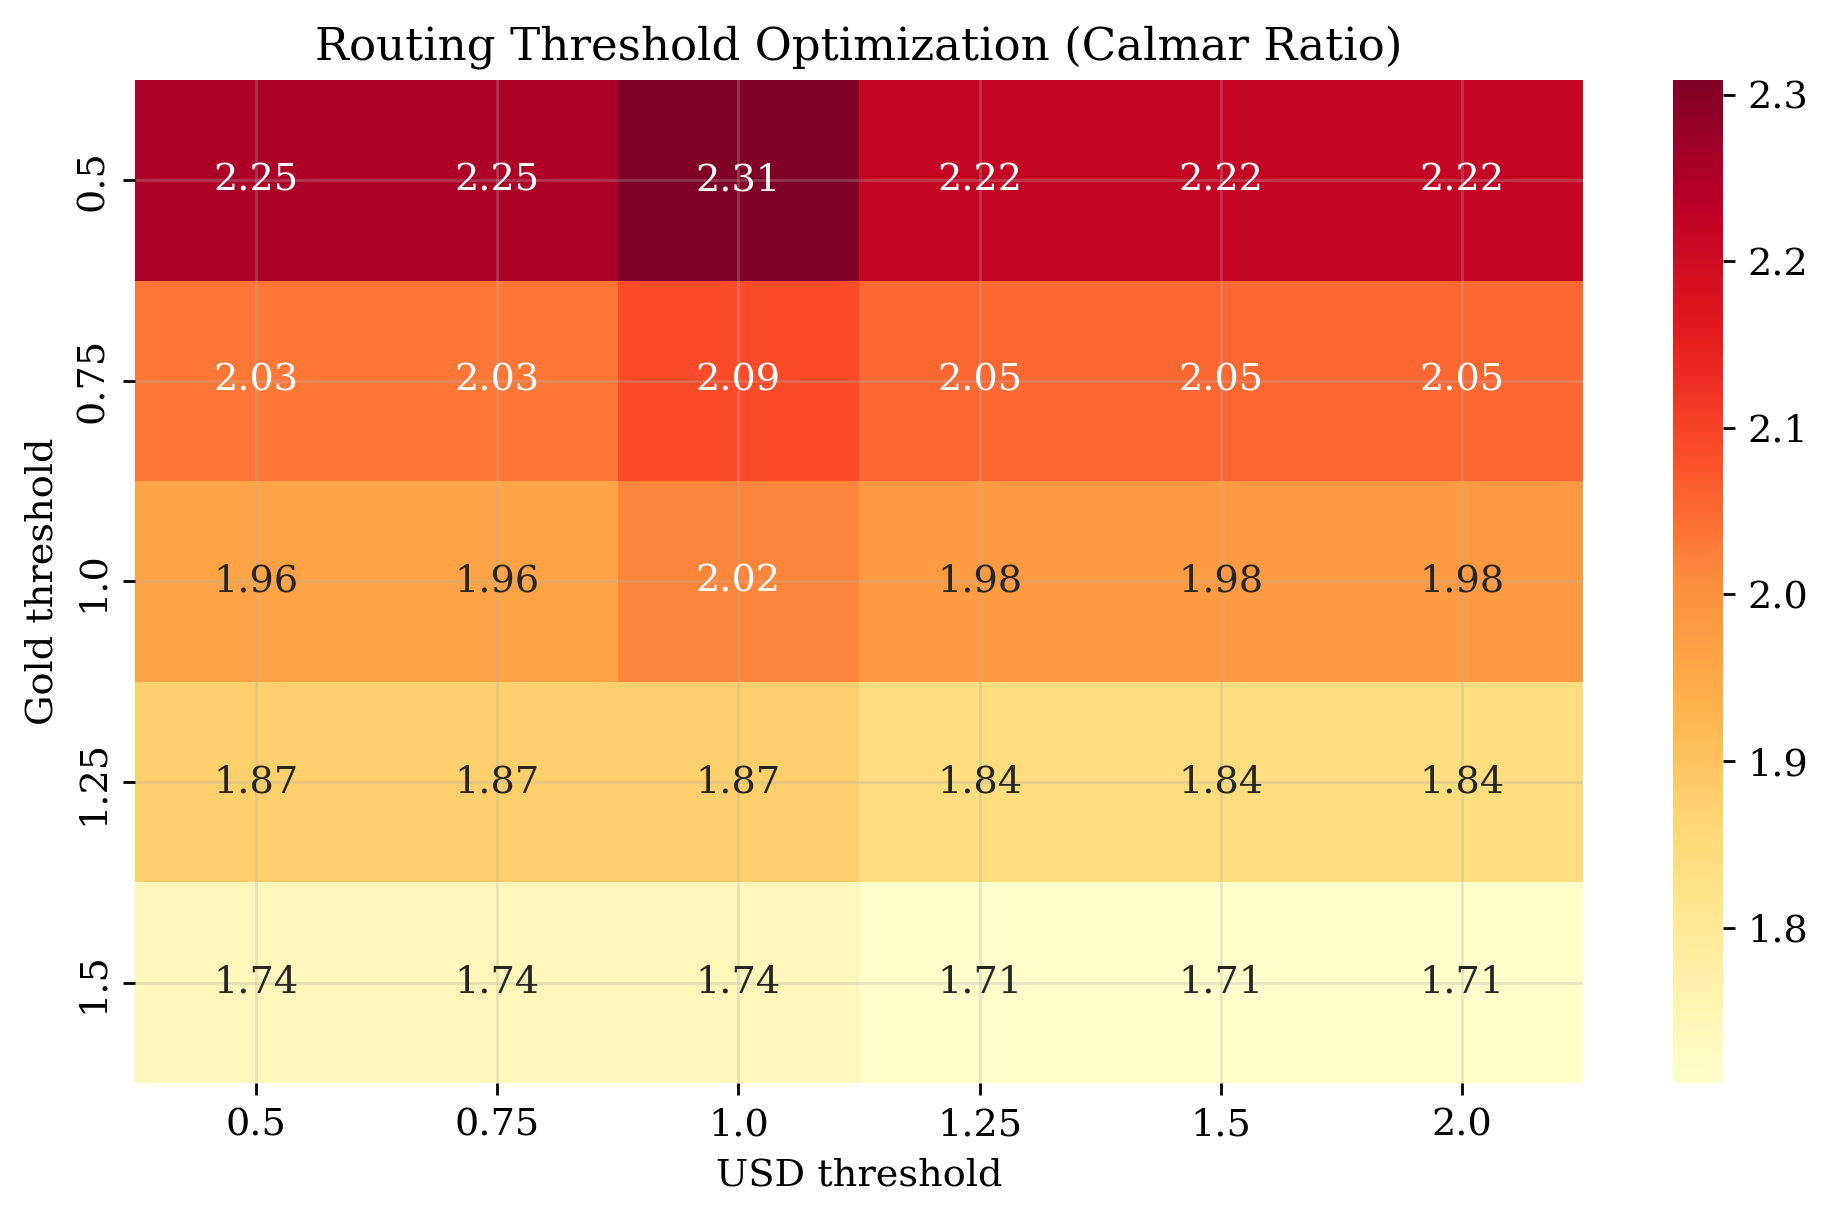
\includegraphics[width=\textwidth]{figures/fig_calmar_heatmap.png}\\[0.2cm]
  \footnotesize
  Grid search over $\tau_{\text{USD}} \times \tau_{\text{Gold}}$. Calmar ratio weighted by fold duration. Optimal: $\tau_u = 1.0$, $\tau_g = 0.5$. The gold threshold is lower because gold signals are less frequent but more persistent.
\end{column}
\begin{column}{0.50\textwidth}
  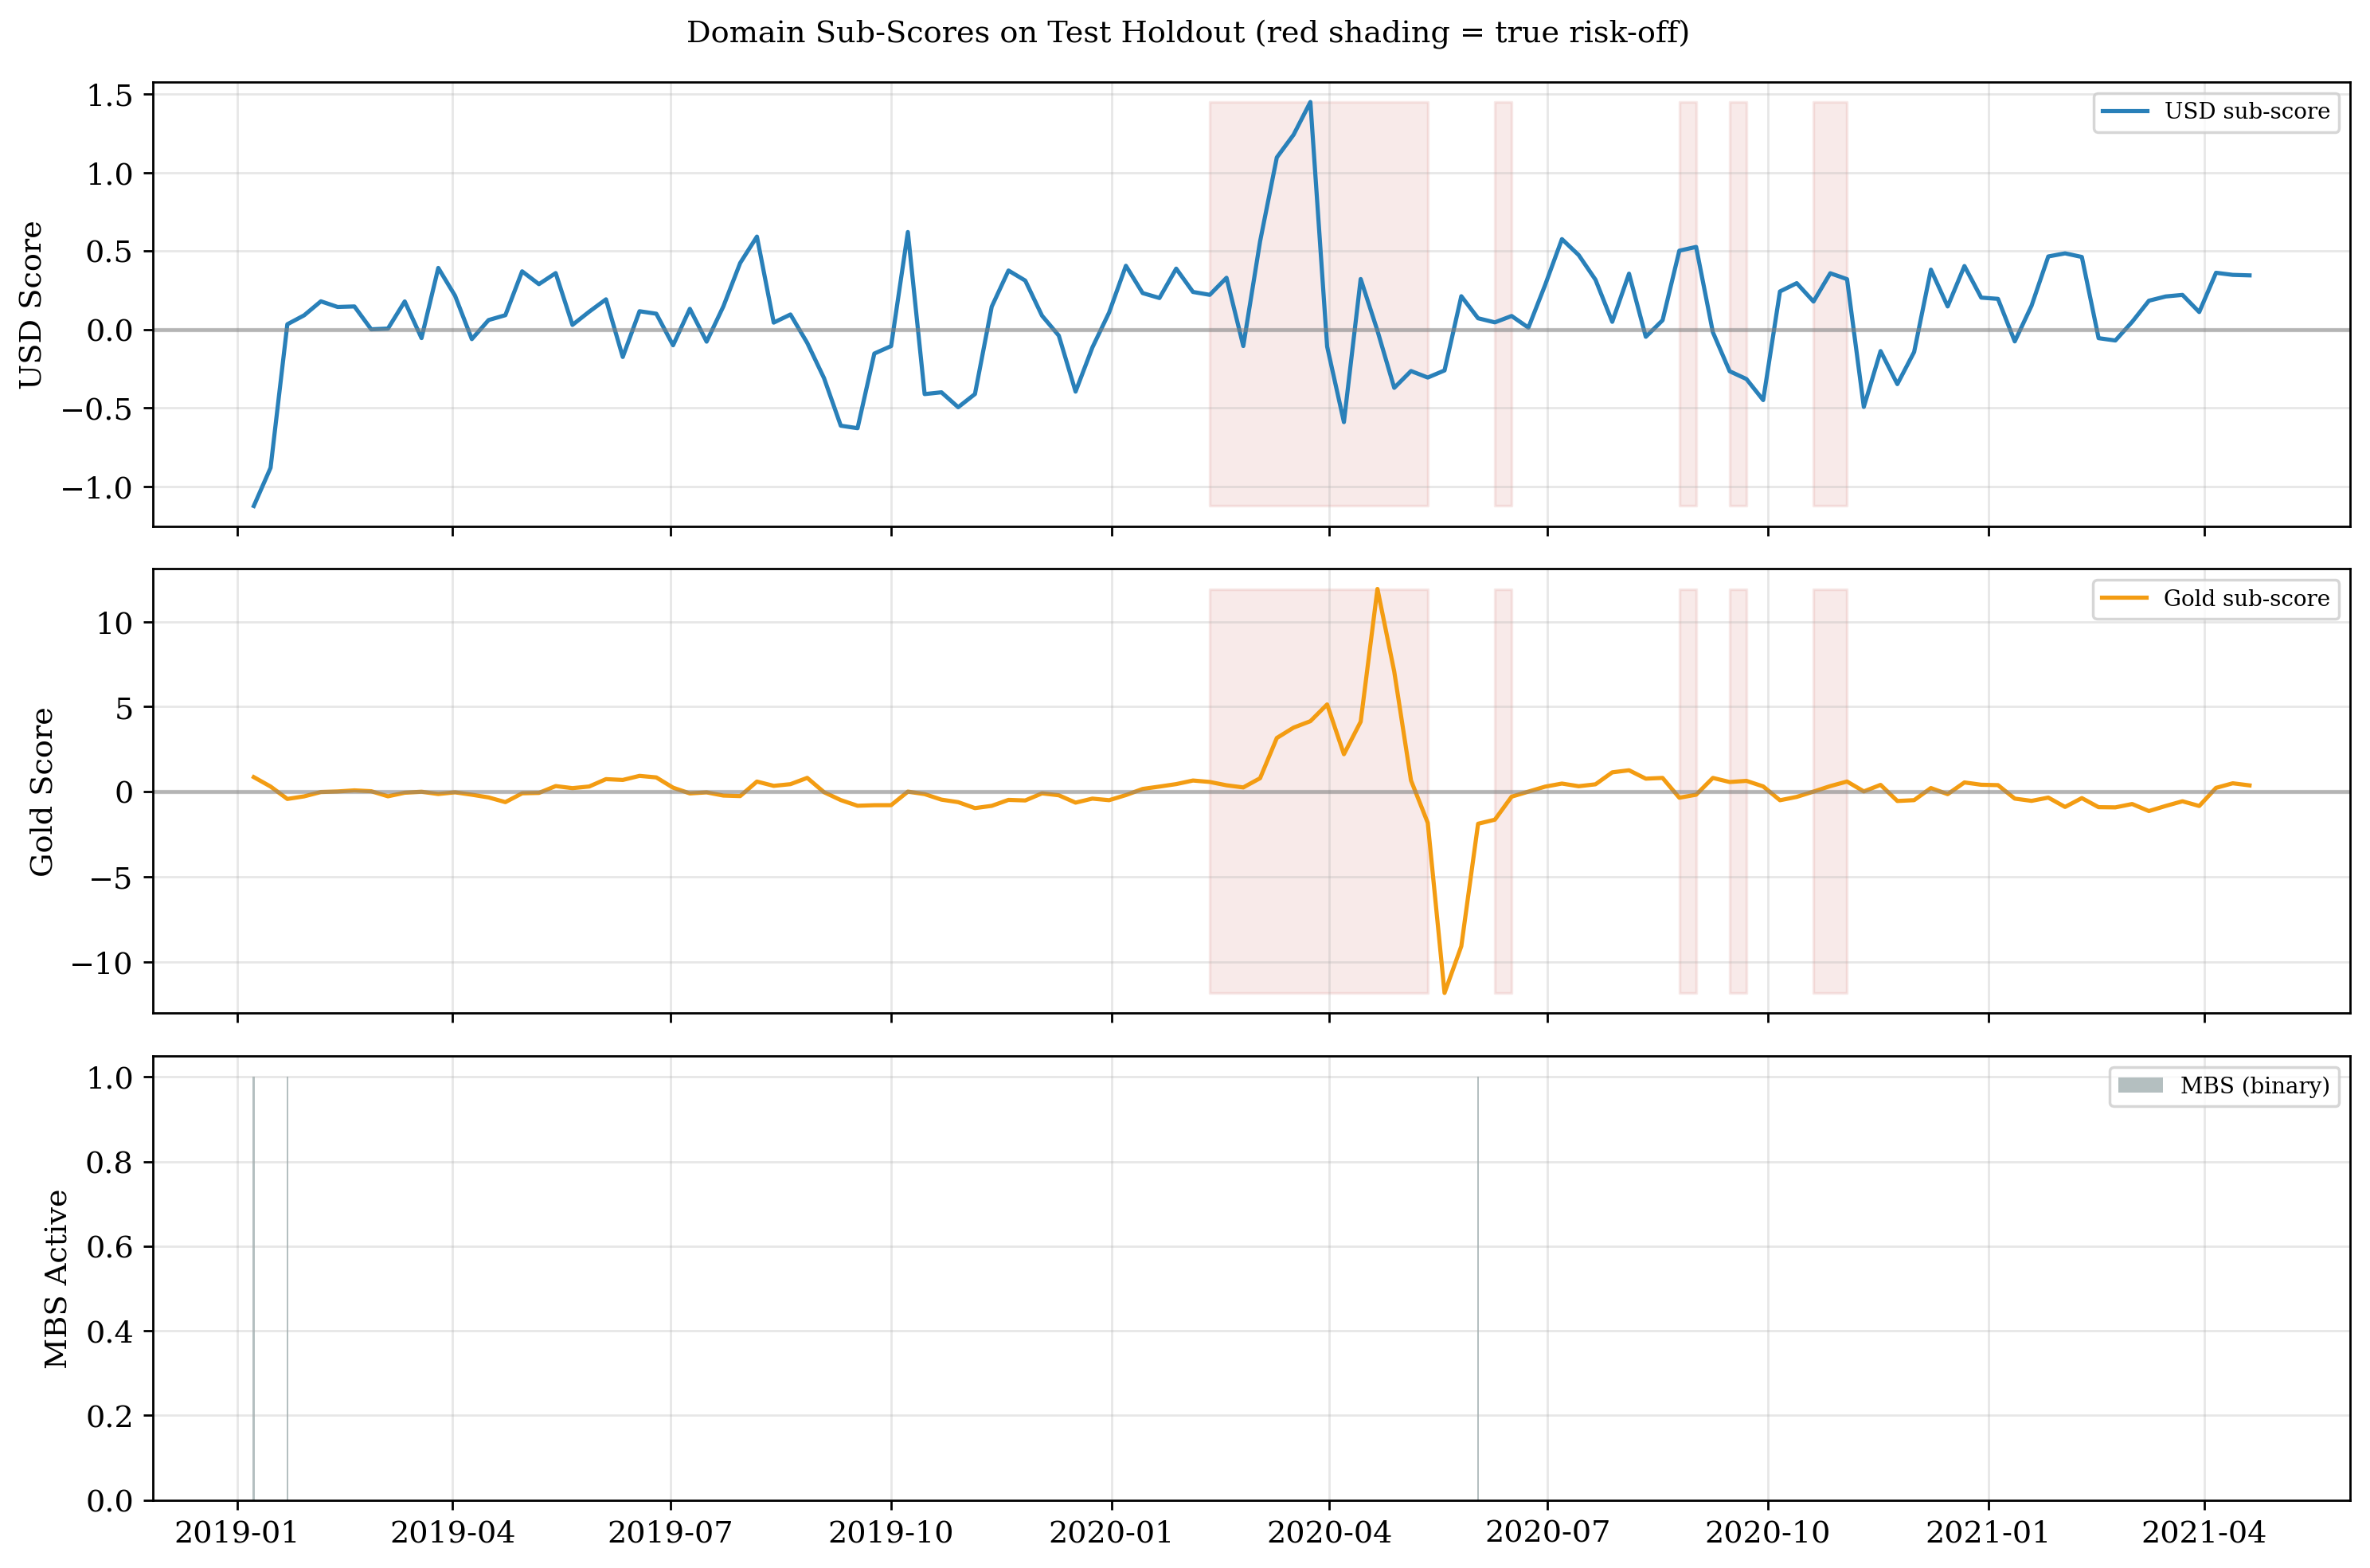
\includegraphics[width=\textwidth]{figures/fig_subscores.png}\\[0.1cm]
  \footnotesize
  \textbf{Top:} USD sub-score spikes during COVID crash (funding stress). \textbf{Middle:} Gold sub-score elevated during COVID and recovery (stimulus, low real yields). \textbf{Bottom:} MBS activates only once (strict conditions).\\[0.1cm]
  Red shading = true risk-off. Sub-scores provide \textbf{interpretable} routing --- you can trace which macro regime drove each allocation.
\end{column}
\end{columns}
\end{frame}

% ── SLIDE 15: LIMITATIONS & CONCLUSIONS ──
\begin{frame}{Limitations, Conclusions \& Future Work}
\begin{columns}[T]
\begin{column}{0.48\textwidth}
  \textbf{Limitations (candidly):}
  \begin{itemize}\setlength\itemsep{0.08cm}
    \footnotesize
    \item \textbf{Short test period:} 120 weeks, 9 regime switches --- results depend on few trades; not yet statistically robust
    \item \textbf{Thin CV folds:} Folds 3--5 have 2--10 positives; $n_{\text{pos}}$-weighting mitigates but doesn't eliminate noise
    \item \textbf{Proxy constraints:} MXUS $\neq$ MSCI World; log-ratios $\neq$ credit spreads
    \item \textbf{Weekly frequency:} misses intra-week volatility events
    \item \textbf{No 2022 data:} the inflation/rate shock regime --- the true test for Gold routing --- is absent
    \item \textbf{Leverage risk:} at 1.5$\times$, a \textit{missed} crisis costs more; the system's 35\% recall gap is a genuine concern
  \end{itemize}
\end{column}
\begin{column}{0.48\textwidth}
  \textbf{Conclusions:}
  \begin{itemize}\setlength\itemsep{0.08cm}
    \footnotesize
    \item The \textbf{ensemble of unsupervised detectors} outperforms all single models (F1 0.65 vs.\ 0.62 best single)
    \item \textbf{Domain-specific routing} adds genuine intelligence vs.\ binary risk-on/off
    \item \textbf{Walk-forward + embargo} provides methodologically sound OOS evaluation
    \item Strategy achieves \textbf{Sharpe 1.93} with \textbf{Max DD $-$12\%} vs.\ $-$28\% for buy\&hold
  \end{itemize}
  \vspace{0.2cm}
  \textbf{Future work:}
  \begin{itemize}\setlength\itemsep{0.05cm}
    \footnotesize
    \item Daily frequency for finer granularity
    \item SHAP / Mahalanobis decomposition for signal attribution
    \item Include 2022--2025 data (inflation regime)
    \item Regime-switching models (HMM) as benchmark
    \item Bootstrap CV for confidence intervals
  \end{itemize}
\end{column}
\end{columns}
\end{frame}

\end{document}
